% --------------------------------------------------------------
% This is all preamble stuff that you don't have to worry about.
% Head down to where it says "Start here"
% --------------------------------------------------------------
\documentclass[12pt]{article}
\usepackage[spanish]{babel}
\usepackage[utf8x]{inputenc}
\usepackage{amsmath}
\usepackage{graphicx}
\usepackage[colorinlistoftodos]{todonotes}
\usepackage{color}
\usepackage{subfigure}
\usepackage{enumitem}
\usepackage{algpseudocode}
\usepackage{float}
\usepackage{enumerate}


\usepackage{listings}
\lstset{language=Octave} % https://v2.overleaf.com/7342361719drzgtrhtknsj

\providecommand{\abs}[1]{\lvert#1\rvert}
\providecommand{\norm}[1]{\lVert#1\rVert}
\sloppy
\definecolor{lightgray}{gray}{0.5}
\setlength{\parindent}{0pt}
\usepackage[margin=1in]{geometry} 
\usepackage{amsmath,amsthm,amssymb}
 
\newcommand{\N}{\mathbb{N}}
\newcommand{\Z}{\mathbb{Z}}
 
\newenvironment{theorem}[2][Theorem]{\begin{trivlist}
\item[\hskip \labelsep {\bfseries #1}\hskip \labelsep {\bfseries #2.}]}{\end{trivlist}}
\newenvironment{lemma}[2][Lemma]{\begin{trivlist}
\item[\hskip \labelsep {\bfseries #1}\hskip \labelsep {\bfseries #2.}]}{\end{trivlist}}
\newenvironment{exercise}[2][Exercise]{\begin{trivlist}
\item[\hskip \labelsep {\bfseries #1}\hskip \labelsep {\bfseries #2.}]}{\end{trivlist}}
\newenvironment{reflection}[2][Reflection]{\begin{trivlist}
\item[\hskip \labelsep {\bfseries #1}\hskip \labelsep {\bfseries #2.}]}{\end{trivlist}}
\newenvironment{proposition}[2][Proposition]{\begin{trivlist}
\item[\hskip \labelsep {\bfseries #1}\hskip \labelsep {\bfseries #2.}]}{\end{trivlist}}
\newenvironment{corollary}[2][Corollary]{\begin{trivlist}
\item[\hskip \labelsep {\bfseries #1}\hskip \labelsep {\bfseries #2.}]}{\end{trivlist}}
 
\begin{document}
 
% --------------------------------------------------------------
%                         Start here
% --------------------------------------------------------------
 
%\renewcommand{\qedsymbol}{\filledbox}

\title{Trabajo de estatica en \LaTeX}

\author{Beicker Baena Baldiris \and Yeison Sarmiento Lopez \and Yair Franco Puello \and 'Alvaro Polo Ulloque\and\ Dayana Jimenez Perez} 

\begin{titlepage}

\newcommand{\HRule}{\rule{\linewidth}{0.5mm}} % Defines a new command for the horizontal lines, change thickness here

\center % Center everything on the page
 
%----------------------------------------------------------------------------------------
%	HEADING SECTIONS
%----------------------------------------------------------------------------------------

\textsc{\LARGE Universidad Cat\'olica San pablo}\\[1.5cm] % Name of your university/college
\textsc{\Large Matem\'atica para la Computaci\'on}\\[0.5cm] % Major heading such as course name
\textsc{\large }\\[0.5cm] % Minor heading such as course title

%----------------------------------------------------------------------------------------
%	TITLE SECTION
%----------------------------------------------------------------------------------------

\HRule \\[0.4cm]
{ \huge \bfseries Lista de Ejercicios Nro.3 }\\[0.4cm] % Title of your document
\HRule \\[1.5cm]
 
%----------------------------------------------------------------------------------------
%	AUTHOR SECTION
%----------------------------------------------------------------------------------------

\begin{minipage}{0.4\textwidth}
\begin{flushleft} \large
\emph{Entregado por:}\\
\begin{itemize}
    \item Victor Flores
\item  Daniel Palomino
\item Solange Ramos
\item Felipe Moreno
\item David Choqueluque
\end{itemize}
\end{flushleft}
\end{minipage}
~
\begin{minipage}{0.4\textwidth}
\begin{flushright} \large
\emph{Profesor:} \\
Sergio \textsc{Aquise Escobedo} % Supervisor's Name
\end{flushright}
\end{minipage}\\[2cm]

% If you don't want a supervisor, uncomment the two lines below and remove the section above
%\Large \emph{Author:}\\
%John \textsc{Smith}\\[3cm] % Your name

%----------------------------------------------------------------------------------------
%	DATE SECTION
%----------------------------------------------------------------------------------------

{\large \today}\\[2cm] % Date, change the \today to a set date if you want to be precise

\vfill % Fill the rest of the page with whitespace

\end{titlepage}

\newpage

\section{Implemente los siguientes códigos}
\subsection{La solución de un sistema de ecuaciones lineales usando el método de sobre relajación (SOR)}
%\input{implemente/a.tex} 

%=====================(Solution)==========================

\lstinputlisting{code/SOR.m}

\subsection{Resolver el ejemplo numérico usando el seudocódigo de la página 610 capitulo 15
Ecuaciones diferenciales parciales, el método iterativo de Gauss-Seidel, del libro David
Kinkaid del dropbox}
\textbf{Ejemplo Númerico}: Vamos a ilustrar este procedimiento en el problema con valores en la frontera
\begin{align*}
    \bigtriangledown^2u-\frac{1}{25}u &= 0 \quad dentro de R (cuadrado unitario) \\
    q &= 0 \quad en la frontera de R.
\end{align*}
    donde $q = \cosh 15 x + \cosh 15$ y . De este problema conocemos la solución $u = q$. Se presenta a
continuación un pseudocódigo de controlador para el procedimiento de Gauss-Seidel, comenzando
con $u = 1$ y tomando 20 iteraciones. Considere que sólo se necesitan 81 palabras para el arreglo en
la solución iterativa del sistema lineal de 49 x 49. Aquí, $h = \frac{1}{8}$.
\\
Para este problema modelo, la función principal es:
\\
\lstinputlisting{code/codeGausSeidel/Eliptico.m}

y las funciones acompañantes se muestran acontinaución :
funcion Gaus Seidel\\
\lstinputlisting{code/codeGausSeidel/Seidel.m}

otras funciones\\

\lstinputlisting{code/codeGausSeidel/f.m}

\lstinputlisting{code/codeGausSeidel/g.m}

\lstinputlisting{code/codeGausSeidel/Bndy.m}

\lstinputlisting{code/codeGausSeidel/ustart.m}

\lstinputlisting{code/codeGausSeidel/TrueSolution.m}

%=========================================================

%=========================================================
% BISWA DATA
%=========================================================
% 
% Sección 6.3
% °°°°°°°°°°°°°°°°°°°°°°°°°°°°°°°°°°°°°°°°°°°°°°°°°°°°°°°°
\section{Biswa Datta: Sección 6.3}

% Ejercicio 4
\subsection{Ejercicio 4}
Usando la ecuación de diferencia, construir un sistema lineal para las distribuciones de calor en los siguientes puntos interior de la placa calentada cuyos temperaturas al borde se mantienen constantes.

\begin{center}
    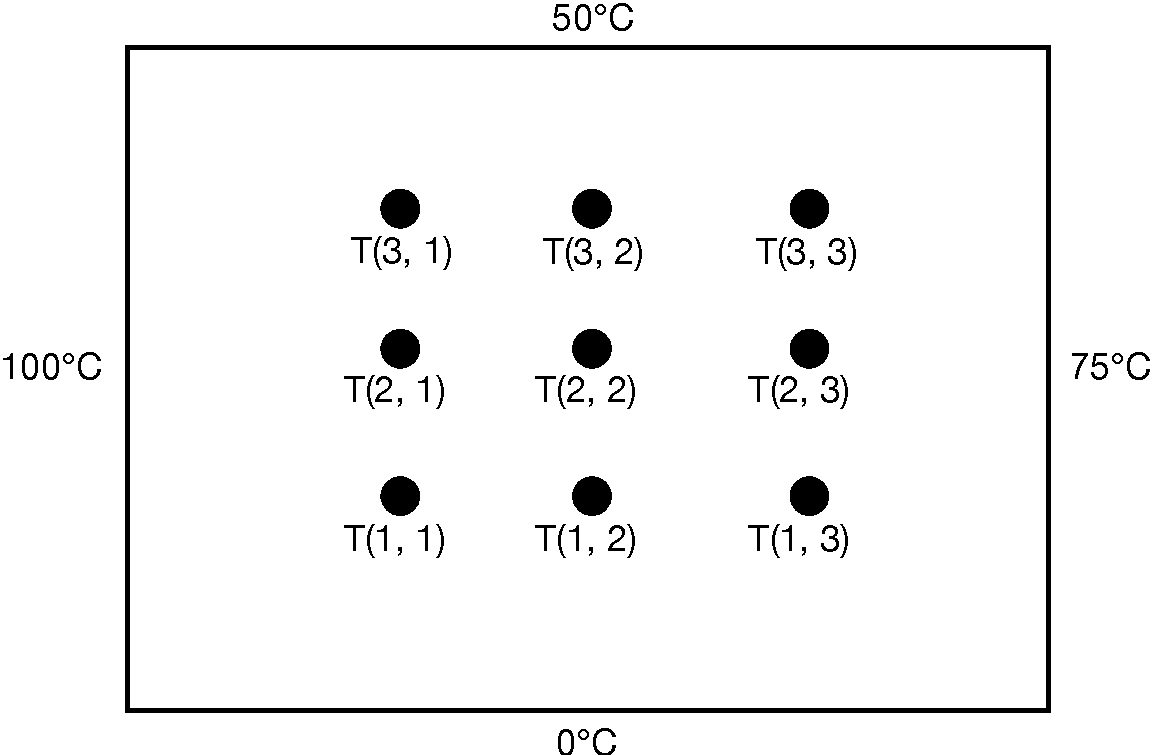
\includegraphics[scale=0.5]{images/heatingmap.pdf}    
\end{center}

Para la discretización de la placa usaremos un \textit{stencil} para generar el sistema:

\begin{center}
    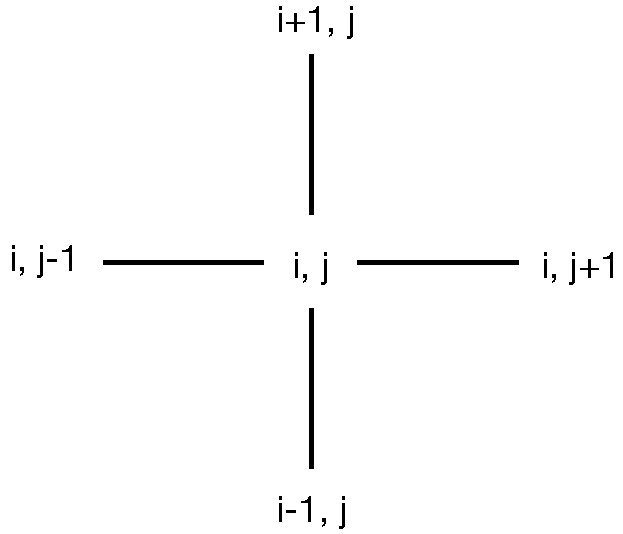
\includegraphics[scale=0.5]{images/stencil.pdf}
\end{center}

La ecuación en diferencias que describe éste \textit{stencil} (discretización de la ecuación elíptica) es la siguiente:

\begin{align}
    \frac{T_{i,j+1} + T_{i,j-1} + T_{i+1,j} + T_{i-1,j} - 4 \times T_{i, j}}{h^2} = 0
\end{align}

Usando éste \textit{stencil}, tendremos que al aplicarlo sobre la grilla $3 \times 3$ en la cual se ha discretizado la placa tendremos las siguientes 9 ecuaciones:

\begin{align*}
T_{1,2} + T_{1,0} + T_{2,1} + T_{0,1} - 4 \times T_{1, 1} &= 0\\
T_{1,3} + T_{1,1} + T_{2,2} + T_{0,2} - 4 \times T_{1, 2} &= 0\\
T_{1,4} + T_{1,2} + T_{2,3} + T_{0,3} - 4 \times T_{1, 3} &= 0\\
T_{2,2} + T_{2,0} + T_{3,1} + T_{1,1} - 4 \times T_{2, 1} &= 0\\
T_{2,3} + T_{2,1} + T_{3,2} + T_{1,2} - 4 \times T_{2, 2} &= 0\\
T_{2,4} + T_{2,2} + T_{3,3} + T_{1,3} - 4 \times T_{2, 3} &= 0\\
T_{3,2} + T_{3,0} + T_{4,1} + T_{2,1} - 4 \times T_{3, 1} &= 0\\
T_{3,3} + T_{3,1} + T_{4,2} + T_{2,2} - 4 \times T_{3, 2} &= 0\\
T_{3,4} + T_{3,2} + T_{4,3} + T_{2,3} - 4 \times T_{3, 3} &= 0\\
\end{align*}

Aplicando las condiciones de borde, podemos reducir el sistema al siguiente:

\begin{align*}
T_{1,2} + T_{2,1} - 4 \times T_{1, 1} &= - T_{1,0} - T_{0,1} = -0 - 100 = -100\\
T_{1,3} + T_{1,1} + T_{2,2} - 4 \times T_{1, 2} &= -T_{0,2} = -0 = 0\\
T_{1,2} + T_{2,3} - 4 \times T_{1, 3} &= 0 = -T_{1,4} - T_{0,3} = -75 - 0 = -75 \\
T_{2,2} + T_{3,1} + T_{1,1} - 4 \times T_{2, 1} &= -T_{2,0} = -100 \\
T_{2,3} + T_{2,1} + T_{3,2} + T_{1,2} - 4 \times T_{2, 2} &= 0\\
T_{2,2} + T_{3,3} + T_{1,3} - 4 \times T_{2, 3} &= -T_{2,4} = -75\\
T_{3,2} + T_{2,1} - 4 \times T_{3, 1} &= -T_{3,0} - T_{4,1} = -100 -50 = -150\\
T_{3,3} + T_{3,1} + T_{2,2} - 4 \times T_{3, 2} &= -T_{4,2} = -50\\
T_{3,2} + T_{2,3} - 4 \times T_{3, 3} &= -T_{3,4} - T_{4,3} = -75 - 50 = -125\\
\end{align*}

La cual genera el siguiente sistema:

\[
    \begin{bmatrix}
        -4 & 1 & 0 & 1 & 0 & 0 & 0 & 0 & 0 \\
        1 & -4 & 1 & 0 & 1 & 0 & 0 & 0 & 0 \\
        0 & 1 & -4 & 1 & 0 & 1 & 0 & 0 & 0 \\
        1 & 0 & 1 & -4 & 1 & 0 & 1 & 0 & 0 \\
        0 & 1 & 0 & 1 & -4 & 1 & 0 & 1 & 0 \\
        0 & 0 & 1 & 0 & 1 & -4 & 1 & 0 & 1 \\
        0 & 0 & 0 & 1 & 0 & 1 & -4 & 1 & 0 \\
        0 & 0 & 0 & 0 & 1 & 0 & 1 & -4 & 1 \\
        0 & 0 & 0 & 0 & 0 & 1 & 0 & 1 & -4 \\
    \end{bmatrix}
\] 

% Ejercicio 5
\subsection{Ejercicio 5}
Derivar el sistema lineal usando la aproximación de Diferencias Finitas en la ecuación diferencial parcial elíptica:
\begin{center}
  $ \frac{\partial^2 T}{\partial x^2} + \frac{\partial^2 T}{\partial y^2} = f(x,y)$    
\end{center}

El paso de las diferencias son: $ \Delta x = \Delta y = 0.25 $ y las condiciones de frontera son:
\begin{center}
  $T(x,0) = 1-x$\\
  $T(1,y)=y$\\
  $T(0,y)=1$\\
  $T(x,1)=1$    
\end{center}

\textbf{Solución}:

De los datos, obtenemos los dominios del problema [0, 1].

Entonces haciendo diferencias finitas tenemos:
\begin{center}
  $ \frac{\partial^2 T(x_i , y_i)}{\partial x^2} = \frac{T_{i+1,j} - 2 T_{i,j} + T_{i-1,j}}{\Delta x ^2}$\\
  $ \frac{\partial^2 T(x_i , y_i)}{\partial y^2} = \frac{T_{i,j+1} - 2 T_{i,j} + T_{i,j-1}}{\Delta y ^2}$\\
\end{center}

Entonces, por aproximación tenemos que:
\begin{center}
  $f(x,y) = \frac{T_{i+1,j} - 2 T_{i,j} + T_{i-1,j}}{\Delta x ^2} + \frac{T_{i,j+1} - 2 T_{i,j} + T_{i,j-1}}{\Delta y ^2}$\\
  $f(x,y) = \frac{T_{i+1,j} + T_{i-1,j} - 4 T_{i,j} + T_{i,j+1} + T_{i,j-1}}{0.25 ^2} $\\
  $f(x,y) = 16*T_{i+1,j} + 16*T_{i-1,j} - 48* T_{i,j} + 16*T_{i,j+1} + 16*T_{i,j-1} $\\
\end{center}

Como el intervalo es de [0,1] con paso de 0.25, tenemos 16 puntos: 0, 0.25, 0.5, 0.75, 1 en X y Y. Generando una malla en dichos intervalos. \\

De los cuales, faltaría calcular los puntos: (0.25, 0.25), (0.25, 0.5), (0.25, 0.75), (0.5,0.25), (0.5,0.5), (0.5, 0.75), (0.75, 0.25), (0.75, 0.5) y (0.75, 0.75).\\

Los cuales se calculan como:

i=1, j=1(0.25,0.25):\\
$f(x_1,y_1) = 16*T_{2,1} + 16*T_{0,1} - 48 T_{1,1} + 16*T_{1,2} + 16*T_{1,0}$\\

i=1, j=2(0.25,0.5):\\
$f(x_1,y_2) = 16*T_{2,2} + 16*T_{0,2} - 48 T_{1,2} + 16*T_{1,3} + 16*T_{1,1}$\\

i=1, j=3(0.25,0.75):\\
$f(x_1,y_3) = 16*T_{2,3} + 16*T_{0,3} - 48 T_{1,3} + 16*T_{1,4} + 16*T_{1,2}$\\

i=2, j=1(0.5,0.25):\\
$f(x_2,y_1) = 16*T_{3,1} + 16*T_{1,1} - 48 T_{2,1} + 16*T_{2,2} + 16*T_{2,0}$\\

i=2, j=2(0.5,0.5):\\
$f(x_2,y_2) = 16*T_{3,2} + 16*T_{1,2} - 48 T_{2,2} + 16*T_{2,3} + 16*T_{2,1}$\\

i=2, j=3(0.5,0.75):\\
$f(x_2,y_3) = 16*T_{3,3} + 16*T_{1,3} - 48 T_{2,3} + 16*T_{2,4} + 16*T_{2,2}$\\

i=3, j=1(0.5,0.25):\\
$f(x_3,y_1) = 16*T_{4,1} + 16*T_{2,1} - 48 T_{3,1} + 16*T_{3,2} + 16*T_{3,0}$\\

i=3, j=2(0.5,0.5):\\
$f(x_3,y_2) = 16*T_{4,2} + 16*T_{2,2} - 48 T_{3,2} + 16*T_{3,3} + 16*T_{3,1}$\\

i=3, j=3(0.5,0.75):\\
$f(x_3,y_3) = 16*T_{4,3} + 16*T_{2,3} - 48 T_{3,3} + 16*T_{3,4} + 16*T_{3,2}$\\

Calculando los respectivos valores:

$T_{0,1} = T(0, 0.25) = 1 $, $T_{4,1} = T(1,0.25) = 0.25$\\
$T_{0,2} = T(0, 0.5) = 1$, $T_{4,2} = T(1,0.5) = 0.5 $\\
$T_{0,3} = T(0, 0.75) = 1$, $T_{4,3} = T(1,0.75) = 0.75 $\\
$T_{1,0} = T(0.25, 0) = 0.75$, $T_{2,0} = T(0.5, 0) = 0.5$, $T_{3,0} = T(0.75, 0) = 0.25$\\
$T_{1,4} = T(0.25, 1) = 1$, $T_{2,4} = T(0.5,1) = 1$, $T_{3,4} = T(0.75,1) = 1$\\
\\Solo quedaría calcular los puntos:

$T_{1,1} $, $T_{2,1} $, $T_{3,1} $\\
$T_{1,2}$, $T_{2,2} $, $T_{3,2} $\\
$T_{1,3} $, $T_{2,3} $, $T_{3,3} $\\
\\Los cuales se obtiene de la solución del sistema de ecuaciones formado arriba, el cual se expresa de la siguiente manera:

$f(x_1,y_1) = 16*T_{2,1} + 16 - 48 T_{1,1} + 16*T_{1,2} + 16*0.25$\\
$f(x_1,y_2) = 16*T_{2,2} + 16 - 48 T_{1,2} + 16*T_{1,3} + 16*T_{1,1}$\\
$f(x_1,y_3) = 16*T_{2,3} + 16 - 48 T_{1,3} + 16 + 16*T_{1,2}$\\
$f(x_2,y_1) = 16*T_{3,1} + 16*T_{1,1} - 48 T_{2,1} + 16*T_{2,2} + 16*0.5$\\
$f(x_2,y_2) = 16*T_{3,2} + 16*T_{1,2} - 48 T_{2,2} + 16*T_{2,3} + 16*T_{2,1}$\\
$f(x_2,y_3) = 16*T_{3,3} + 16*T_{1,3} - 48 T_{2,3} + 16 + 16*T_{2,2}$\\
$f(x_1,y_1) = 16*0.25 + 16*T_{2,1} - 48 T_{3,1} + 16*T_{3,2} + 16*0.25$\\
$f(x_2,y_2) = 16*0.5 + 16*T_{2,2} - 48 T_{3,2} + 16*T_{3,3} + 16*T_{3,1}$\\
$f(x_3,y_3) = 16*0.75 + 16*T_{2,3} - 48 T_{3,3} + 16 + 16*T_{3,2}$\\

Dandole una forma de Matrices y vectores tenemos:
\[
\begin{bmatrix}
    -48 & 16 & 0 & 16 & 0 & 0 & 0 & 0\\
    16 & -48 & 16 & 0 & 16 & 0 & 0 & 0 & 0 \\
    0 &  0 & -48 & 16 & 0 & 16 & 0 & 0 & 0 \\
    16 & 0 & 0 & -48 & 16 & 0 & 16 & 0 & 0 \\
    0 & 16 & 0 & 16 & -48 & 16 & 0 & 16 & 0 \\
    0 & 0 & 16 & 0 & 16 & -48 & 0 & 0 & 16  \\
    0 & 0 & 0& 16 & 0 & 0 & -48 & 16 & 0\\
    0 & 0 & 0 & 0 & 16 & 0 & 16 & -48 & 16 \\
    0 & 0 & 0 & 0 & 0 & 16 & 0 & 16 & -48 \\
\end{bmatrix}
+
\begin{bmatrix}
    T_{1,1} \\
    T_{1,2} \\
    T_{1,3} \\
    T_{2,1} \\
    T_{2,2} \\
    T_{2,3} \\
    T_{3,1} \\
    T_{3,2} \\
    T_{3,3} 
\end{bmatrix}
=
\begin{bmatrix}
    f(0.25, 0.25) - 20 \\
    f(0.25, 0.5) - 16\\
    f(0.25, 0.75) - 32\\
    f(0.5, 0.25) - 8\\
    f(0.5, 0.5) \\
    f(0.5, 0.75) - 16\\
    f(0.75, 0.25) -8 \\
    f(0.75, 0.5) - 8 \\
    f(0.75, 0.75) - 28 \\
\end{bmatrix}
\]

Como se puede observar, se generó una matriz pentadiagonal (2 vecinos iguales de la diagonal), para resolver dicha ecuación depende exclusivamente de la función f(x,y). 

% Ejercicio 6
\subsection{Ejercicio 6}
Para el sistema del problema anterior, si
\begin{gather*}
f(x,y) = -\pi^{2} sin( \pi x ) sin( \pi y )
\end{gather*}
la solución analítica a la ecuación elíptica
\begin{gather*}
\frac{\partial^{2} T}{\partial x^{2}} + \frac{\partial^{2} T}{\partial y^{2}} = f(x,y)
\end{gather*}
con las mismas condiciones de frontera como en el problema anterior, es dada por:
\begin{gather*}
T(x,y) = 1 - x + xy + 0.5 sin( \pi x ) sin( \pi y )
\end{gather*}

\begin{itemize}
\item[$(a)$] Use el método de diferencias finitas para aproximar $T$ en el interior de los puntos con $\Delta x = \Delta y = 1 / n$, con $n=4,8,16$\\
\textbf{\underline{Solución:}}

Para esto definimos el siguiente script en Matlab, el cual nos permitirá discretizar y resolver el sistema dado.

\lstset{language=Matlab}
\begin{lstlisting}[frame=single]
%define the domain of the problem
LX = 1;
LY = 1;

%define the level of discretization
n = 16;
DX = LX / n;
DY = LY / n;

%define our system
nx = n + 1;
ny = n + 1;

dim = ( ny - 2 ) * ( nx - 2 );

[sysMat,sysVec] = generateGrid( nx, ny, dim, DX, DY );

sysSol = sysMat \ sysVec;

%disp( 'system matrix' );
disp( sysMat );
%disp( 'system vector' );
disp( sysVec );
disp( 'system solution for n =8' );
%disp( sysSol );
displayColVector( sysSol );

approxSolMat = matFromVectorSolution( sysSol, nx, ny );
exactSolMat  = exactSolutionMat( nx, ny, DX, DY );
disp( 'approx solution' )
disp( approxSolMat )
disp( 'exact solution' )
disp( exactSolMat )

displayHeatmap( sysSol, nx, ny, DX, DY );

%define helper functions

function plateTempMat = exactSolutionMat( nx, ny, DX, DY )
    plateTempMat = zeros( nx - 2, ny - 2);
    for i = 1:( nx - 2 )
        for j = 1:( ny - 2 )
            x = j * DX;
            y = i * DY;
            plateTempMat( i, j ) = 1 - x + x * y + ...
		   0.5 * sin( pi * x ) * sin( pi * y );
        end
    end
    plateTempMat = flip( plateTempMat );
end

function plateTempMat = matFromVectorSolution(solVector, nx, ny)
    plateTempMat = reshape( solVector, nx - 2, ny - 2 );
    plateTempMat = plateTempMat';
    plateTempMat = flip( plateTempMat );
end

function displayHeatmap( solution, nx, ny, DX, DY )
    appSol = matFromVectorSolution( solution, nx, ny );
    extSol = exactSolutionMat( nx, ny, DX, DY );
    figure(1);
    imagesc( appSol );
    colorbar;
    figure(2);
    imagesc( extSol );
    colorbar;
end

function displayColVector( vec )
    v_size = ( size( vec ) );
    n = v_size( 1 );
    for i = 1:n
        fprintf( '%f  ', vec( i ) );
        if mod( i, 10 ) == 0
            fprintf( '\n' );
        end
    end
    fprintf( '\n' );
end

function indxInMat = getIndxInSysMat( i, j, nx ) %#ok<*FNDEF>
    indxInMat = ( i - 1 ) * ( nx - 2 ) + j;
end

function valBoundary = getBoundaryCondition(i,j,nx,ny,DX,DY )
    if ( i == 0 )
        valBoundary = 1.0 - j * DX;
    elseif ( i == ny - 1 )
        valBoundary = 1.0;
    elseif ( j == 0 )
        valBoundary = 1.0;
    elseif ( j == nx - 1 )
        valBoundary = i * DY;
    else
        disp( 'shouldnt get here :( ' )
        valBoundary = 0;
    end
end

function fxy = f( i, j, DX, DY )
    x = j * DX;
    y = i * DY;
    fxy = -pi^2 * sin( pi * x ) * sin( pi * y ) * DX * DX;
end

function [sysMat,sysVec] = applyStencil( i, j, nx, ny, ...
                                     DX, DY, sysMat, sysVec )
    
    s_row = getIndxInSysMat( i, j, nx );
    % Generate the corresponding row
    % Apply reduced stencil to generate the row of the matrix ...
    % because the i or j if extreme are boundary conditions

    if ( i == 1 )
        if ( j == 1 )
            % bottom left corner
            center_col = s_row;
            right_col  = getIndxInSysMat( i, j + 1, nx );
            up_col     = getIndxInSysMat( i + 1, j, nx );

            sysMat( s_row, center_col ) = -4;
            sysMat( s_row, right_col )  = 1;
            sysMat( s_row, up_col )     = 1;

            sysVec( s_row, 1 ) = f( i, j, DX, DY ) - ...
                                 getBoundaryCondition( i - 1, j, ...
                                                       nx, ny, ...
                                                       DX, DY ) - ...
                                 getBoundaryCondition( i, j - 1, ...
                                                       nx, ny, ...
                                                       DX, DY );

        elseif ( j == nx - 2 )
            % bottom right corner
            center_col = s_row;
            left_col   = getIndxInSysMat( i, j - 1, nx );
            up_col     = getIndxInSysMat( i + 1, j, nx );

            sysMat( s_row, center_col ) = -4;
            sysMat( s_row, left_col )   = 1;
            sysMat( s_row, up_col )     = 1;

            sysVec( s_row, 1 ) = f( i, j, DX, DY ) - ...
                                 getBoundaryCondition( i - 1, j,...
                                                       nx, ny,...
                                                       DX, DY ) - ...
                                 getBoundaryCondition( i, j + 1,...
                                                       nx, ny,...
                                                       DX, DY );
        else
            % bottom side
            center_col = s_row;
            left_col   = getIndxInSysMat( i, j - 1, nx );
            right_col  = getIndxInSysMat( i, j + 1, nx );
            up_col     = getIndxInSysMat( i + 1, j, nx );

            sysMat( s_row, center_col ) = -4;
            sysMat( s_row, left_col )   = 1;
            sysMat( s_row, right_col )  = 1;
            sysMat( s_row, up_col )     = 1;

            sysVec( s_row, 1 ) = f( i, j, DX, DY ) - ...
                                 getBoundaryCondition( i - 1, j,...
                                                       nx, ny,...
                                                       DX, DY );
        end
    elseif ( i == ny - 2 )
        
        if ( j == 1 )
            % top left corner
            center_col = s_row;
            right_col  = getIndxInSysMat( i, j + 1, nx );
            down_col   = getIndxInSysMat( i - 1, j, nx );

            sysMat( s_row, center_col ) = -4;
            sysMat( s_row, right_col )  = 1;
            sysMat( s_row, down_col )   = 1;

            sysVec( s_row, 1 ) = f( i, j, DX, DY ) - ...
                                 getBoundaryCondition( i + 1, j,...
                                                       nx, ny,...
                                                       DX, DY ) - ...
                                 getBoundaryCondition( i, j - 1,...
                                                       nx, ny,...
                                                       DX, DY );

        elseif ( j == nx - 2 )
            % top right corner
            center_col = s_row;
            left_col   = getIndxInSysMat( i, j - 1, nx );
            down_col   = getIndxInSysMat( i - 1, j, nx );

            sysMat( s_row, center_col ) = -4;
            sysMat( s_row, left_col )   = 1;
            sysMat( s_row, down_col )   = 1;

            sysVec( s_row, 1 ) = f( i, j, DX, DY ) - ...
                                 getBoundaryCondition( i + 1, j,...
                                                       nx, ny,...
                                                       DX, DY ) - ...
                                 getBoundaryCondition( i, j + 1,...
                                                       nx, ny,...
                                                       DX, DY );
        else
            % up side
            center_col = s_row;
            left_col   = getIndxInSysMat( i, j - 1, nx );
            right_col  = getIndxInSysMat( i, j + 1, nx );
            down_col   = getIndxInSysMat( i - 1, j, nx );

            sysMat( s_row, center_col ) = -4;
            sysMat( s_row, left_col )   = 1;
            sysMat( s_row, right_col )  = 1;
            sysMat( s_row, down_col )   = 1;

            sysVec( s_row, 1 ) = f( i, j, DX, DY ) - ...
                                 getBoundaryCondition( i + 1, j,...
                                                       nx, ny,...
                                                       DX, DY );
        end
        
    elseif ( j == 1 )
        % left side
        center_col = s_row;
        up_col     = getIndxInSysMat( i + 1, j, nx );
        right_col  = getIndxInSysMat( i, j + 1, nx );
        down_col   = getIndxInSysMat( i - 1, j, nx );

        sysMat( s_row, center_col ) = -4;
        sysMat( s_row, up_col )     = 1;
        sysMat( s_row, right_col )  = 1;
        sysMat( s_row, down_col )   = 1;

        sysVec( s_row, 1 ) = f( i, j, DX, DY ) - ...
                             getBoundaryCondition( i, j - 1,...
                                                   nx, ny,...
                                                   DX, DY );
           
    elseif ( j == nx - 2 )
        % right side
        center_col = s_row;
        left_col   = getIndxInSysMat( i, j - 1, nx );
        up_col     = getIndxInSysMat( i + 1, j, nx );
        down_col   = getIndxInSysMat( i - 1, j, nx );

        sysMat( s_row, center_col ) = -4;
        sysMat( s_row, left_col )   = 1;
        sysMat( s_row, up_col )     = 1;
        sysMat( s_row, down_col )   = 1;

        sysVec( s_row, 1 ) = f( i, j, DX, DY ) - ...
                             getBoundaryCondition( i, j + 1,...
                                                   nx, ny,...
                                                   DX, DY );

    else
        % Apply the full stencil
        center_col = s_row;
        left_col   = getIndxInSysMat( i, j - 1, nx );
        right_col  = getIndxInSysMat( i, j + 1, nx );
        up_col     = getIndxInSysMat( i + 1, j, nx );
        down_col   = getIndxInSysMat( i - 1, j, nx );

        sysMat( s_row, center_col ) = -4;
        sysMat( s_row, left_col ) = 1;
        sysMat( s_row, right_col ) = 1;
        sysMat( s_row, up_col ) = 1;
        sysMat( s_row, down_col ) = 1;

        sysVec( s_row, 1 ) = f( i, j, DX, DY );
    end
end

function [sysMat, sysVec] = generateGrid( nx, ny, dim, DX, DY )
    disp( 'generating system matrix' );
    sysMat = zeros( dim, dim );
    sysVec = zeros( dim, 1 );
    for i = 1:( ny - 2 )
       for j = 1:( nx - 2 )
          [sysMat,sysVec] = applyStencil( i, j, nx, ny,...
                                          DX, DY,...
                                          sysMat, sysVec ); 
       end
    end
end
\end{lstlisting}

Los resultados del script para $n=4$ son mostrados a continuación:
\begin{lstlisting}
EllipticPDEsolver
generating system matrix
system matrix
matrix([[-4,  1,  0,  1,  0,  0,  0,  0,  0],
        [ 1, -4,  1,  0,  1,  0,  0,  0,  0],
        [ 0,  1, -4,  0,  0,  1,  0,  0,  0],
        [ 1,  0,  0, -4,  1,  0,  1,  0,  0],
        [ 0,  1,  0,  1, -4,  1,  0,  1,  0],
        [ 0,  0,  1,  0,  1, -4,  0,  0,  1],
        [ 0,  0,  0,  1,  0,  0, -4,  1,  0],
        [ 0,  0,  0,  0,  1,  0,  1, -4,  1],
        [ 0,  0,  0,  0,  0,  1,  0,  1, -4]])

system vector
matrix([[-2.0584],
        [-0.9362],
        [-0.8084],
        [-1.4362],
        [-0.6169],
        [-0.9362],
        [-2.3084],
        [-1.4362],
        [-2.0584]])
        
system solution
matrix([[1.0758],
        [0.9973],
        [0.7008],
        [1.2473],
        [1.2765],
        [0.9973],
        [1.2008],
        [1.2473],
        [1.0758]])
\end{lstlisting}

Para los casos $n=8,16$ tenemos la siguientes soluciones :
%
%%Figure-Problem
\begin{figure}[H]
	\centering
	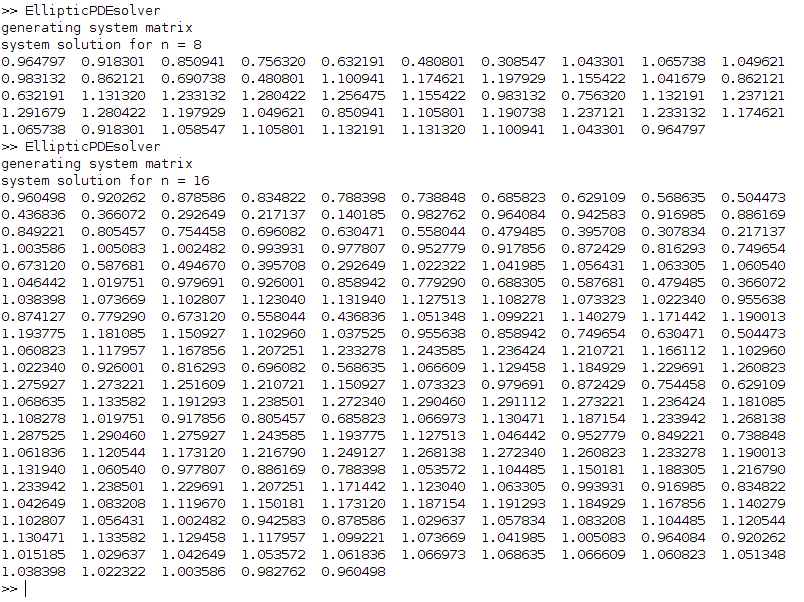
\includegraphics[scale=0.5]{images/img_prob_6_sol_n_8_16.png}
	\caption{Solución del sistema para $n=8$ y $n=16$}
	\label{fig:img_pecc}
\end{figure}
%%%
\item[$(b)$] Comparar los valores obtenidos en el punto anterior con la solución exacta.
\\
Usando el script podemos obtener las siguientes comparaciones de las soluciones aproximada y exacta.
%
%%Figure-Problem
\begin{figure}[H]
	\centering
	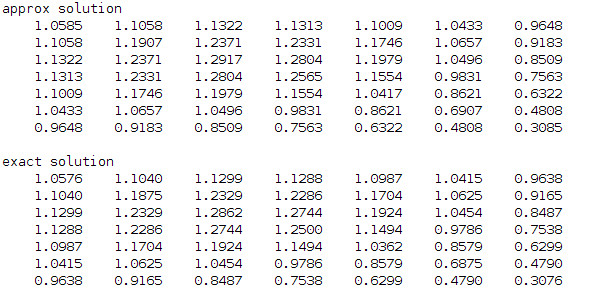
\includegraphics[scale=0.5]{images/img_prob_6_comparison_n8.jpg}
	\caption{Comparación de las soluciones aproximada y exacta para $n=8$}
	\label{fig:img_pecc}
\end{figure}
%%%
%
%%Figure-Problem
\begin{figure}[H]
	\centering
	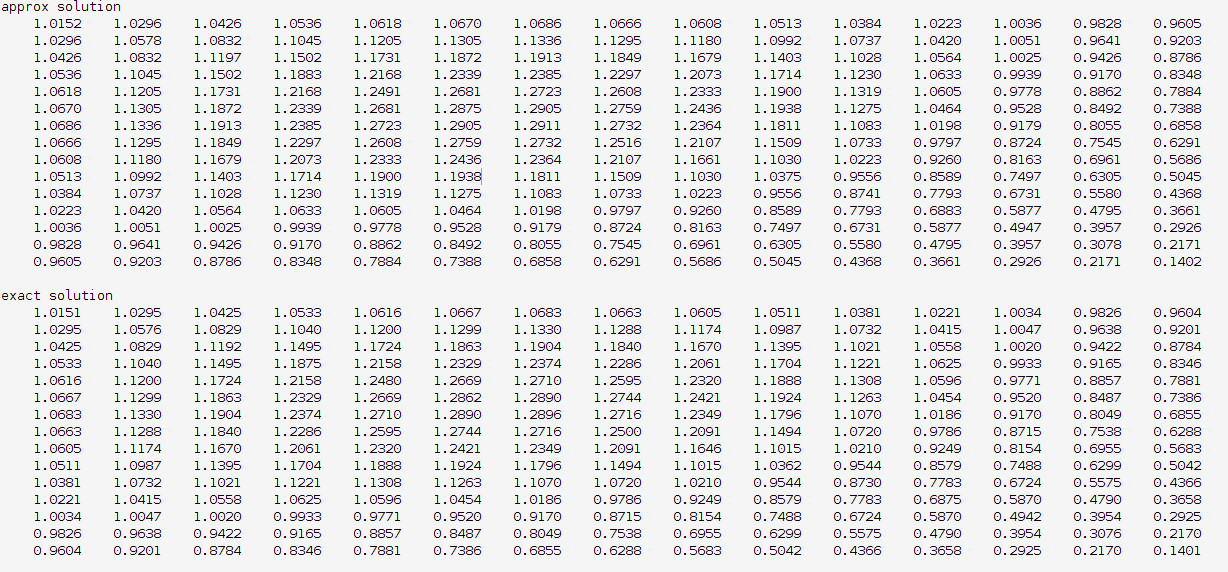
\includegraphics[scale=0.35]{images/img_prob_6_comparison_n16.jpg}
	\caption{Comparación de las soluciones aproximada y exacta para $n=16$}
	\label{fig:img_pecc}
\end{figure}
%%%
%
%%Figure-Problem
\begin{figure}[H]
	\centering
	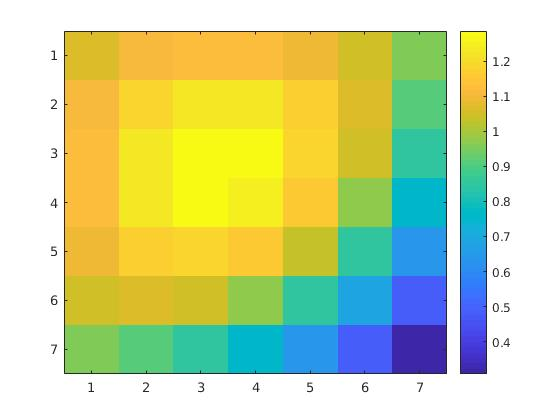
\includegraphics[scale=0.35]{images/img_prob_6_colormap_n8_exact.jpg}
	\caption{Heatmap de la solución exacta para $n=8$}
	\label{fig:img_pecc}
\end{figure}
%%%
%
%%Figure-Problem
\begin{figure}[H]
	\centering
	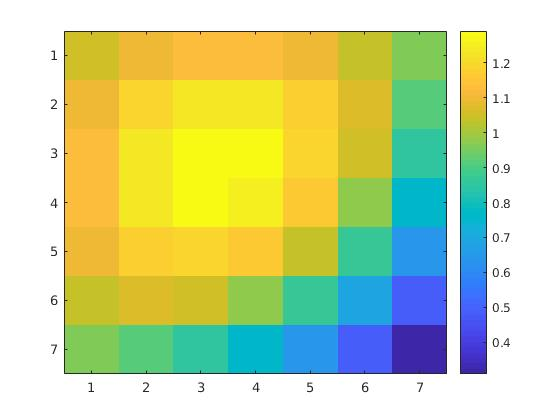
\includegraphics[scale=0.35]{images/img_prob_6_colormap_n8_approx.jpg}
	\caption{Heatmap de la solución aproximada para $n=8$}
	\label{fig:img_pecc}
\end{figure}
%%%
%
%%Figure-Problem
\begin{figure}[H]
	\centering
	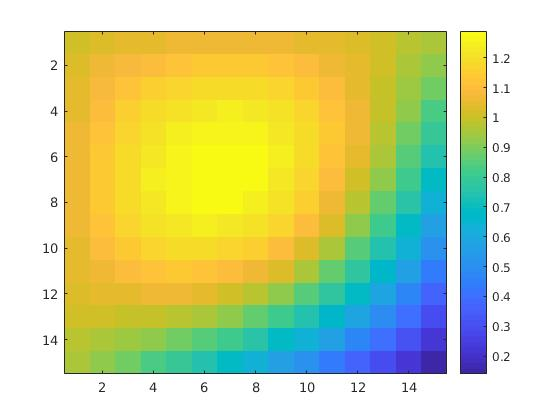
\includegraphics[scale=0.35]{images/img_prob_6_colormap_n16_exact.jpg}
	\caption{Heatmap de la solución exacta para $n=16$}
	\label{fig:img_pecc}
\end{figure}
%%%
%
%%Figure-Problem
\begin{figure}[H]
	\centering
	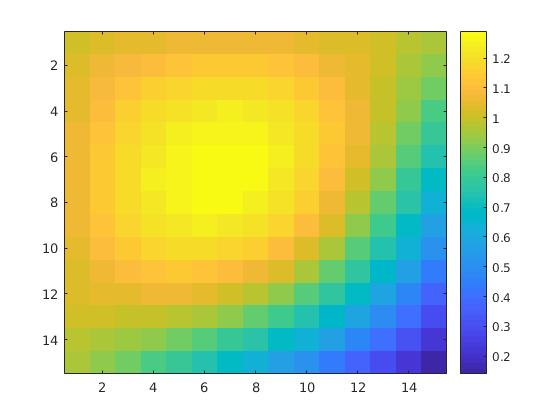
\includegraphics[scale=0.35]{images/img_prob_6_colormap_n16_approx.jpg}
	\caption{Heatmap de la solución aproximada para $n=16$}
	\label{fig:img_pecc}
\end{figure}
%%%
Como se puede observar de las comparaciones, el método devuelve buenas aproximaciones tanto para $n=8$ como para $n=16$.

\item[$(c)$] Defina el sistema lineal resultante al aplicar el metodo de elementos finitos en la solución del problema del valor de frontera de 2 puntos: $-2u''+3u=x^2$, $0\leq x\leq 1$, $u(0)=u(1)=0$,usando malla uniforme y funciones basicas $\phi_j(x)$ como en el libro.\\

\textbf{\underline{Solución:}}

El problema hace referencia a una aproximación por elementos finitos en un entorno 1D tal como se observa en la imagen \ref{2p_mef}.
%%%
%
%%Figure-Problem
\begin{figure}[H]
	\centering
	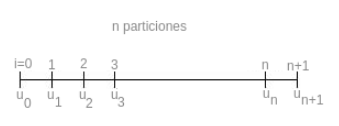
\includegraphics[scale=0.6]{images/2p_bound.png}
	\caption{Representación del problema}
	\label{2p_mef}
\end{figure}
%%%
En el problema se indica las condiciones de frontera en $u_0=0$ y $u_{n+1}=0$. Definiendo sobre el resto de puntos la ecuación usando la aproximación de la derivada  $u''_i=u_{i+1}-2u_i+u_{i-1}$ obtenemos:\\
$$-2.(u_{i+1}-2u_i+u_{i-1})+3u_i=(i/n)^2$$
$$-2.u_{i+1}+7.u_i-2.u_{i-1}=(i/n)^2$$
Remplazando para $i=1,\dots,n$:
$$i=1\to -2u_2+7u_1-2u_0=(1/n)^2$$
$$i=2\to -2u_3+7u_2-2u_1=(2/n)^2$$
$$i=3\to -2u_4+7u_3-2u_2=(3/n)^2$$
$$\vdots$$
$$i=n\to -2u_{n+1}+7u_n-2u_{n-1}=(n/n)^2$$

Usando las ecuaciones de frontera $u_0=0$ y $u_{n+1}=0$ tenemos la forma matricial:\\
\begin{gather*}
\begin{bmatrix}
       7 & -2 & 0 & 0 & \dots & 0 & 0 \\
       -2 & 7 & -2 & 0 & \dots & 0 & 0 \\
       0 & -2 & 7 & -2 & \dots & 0 & 0 \\
       0 & 0 & -2 & 7 & \dots & 0 & 0 \\
       \vdots & \vdots & \vdots & \vdots & \ddots & \vdots & \vdots \\
       0 & 0 & 0 & 0 & \dots & 7 & -2 \\
       0 & 0 & 0 & 0 & \dots & -2 & 7 \\
\end{bmatrix}.
\begin{bmatrix}
    u_1 \\
    u_2 \\
    u_3 \\
    u_4 \\
    \vdots \\
    u_{n-1} \\
    u_n \\
\end{bmatrix}
 = \frac{1}{n^2}.
\begin{bmatrix}
    1^2 \\
    2^2 \\
    3^2 \\
    4^2 \\
    \vdots \\
    (n-1)^2 \\
    n^2 \\
\end{bmatrix}
\end{gather*}



\end{itemize}

% Ejercicio 14
\subsection{Ejercicio 14}
\textbf{Probar que:\\}
    
    \[
        A = \begin{bmatrix}
            4 & -1 & -1 & 0\\
            -1 & 4 & 0 & -1\\
            -1 & 0 & 4 & -1\\
            0 & -1 & -1 & 4\\
        \end{bmatrix}
    \]
    
    es positiva definida con y sin encontrar la factorización de \textit{Cholesky}.\\\\
    
    \textbf{Solución}\\
    
    \textbf{Sin usar Cholesky:}\\
    
    Para que una matriz sea definida positiva, tenemos que probar dos cosas: que sea simétrica y que sus autovalores sean positivos. Como se puede ver, la matriz $A$ es simétrica y sus autovalores son: $\lambda_1 = 2, \lambda_2 = 4, \lambda_3 = 4, \lambda_4 = 6$, todos sus valores positivos. Luego podemos decir que la matriz es positiva definida.\\
        
    \textbf{Cholesky}\\
    
    Debemos encontrar una matriz $H$ tal que $A = H H^T$.
    Para encontrar la matriz usamos las siguientes formulas:
        
        \begin{equation*}
            \begin{split}
                l_{kk} = \sqrt{a_{kk} - \sum_{j=1}^{k-1} l_{kj} ^ 2}\\
                l_{ki} = \frac{a_{ki} - \sum_{j=1}^{i-1} l_{ij} l_{kj} }{l_{ii}}
            \end{split}
        \end{equation*}
        
        Luego la matriz $H$ será:
        
        \[
        H = \begin{bmatrix}
            2 & 0 & 0 & 0\\
            -0.5 & 1.936492 & 0 & 0\\
            -0.5 & -0.129099 & 1.932184 & 0 \\
            0 & -0.516398 & -0.552052 & 1.85164\\
        \end{bmatrix}
       \]
    
    Si multiplicamos $H$ con $H^T$ obtenemos $A$.
 
    \textbf{Resolver el sistema}
    
    \[
        Ax = \begin{bmatrix}
            2\\
            2\\
            2\\
            2\\
        \end{bmatrix}
    \]
    \\\\
    
    \textbf{Solución}\\
    
    Usando $H$ del punto (b), tenemos que:
    \[
        \begin{bmatrix}
            2 & 0 & 0 & 0\\
            -0.5 & 1.936492 & 0 & 0\\
            -0.5 & -0.129099 & 1.932184 & 0 \\
            0 & -0.516398 & -0.552052 & 1.85164\\
        \end{bmatrix} * 
        \begin{bmatrix}
            y_1\\ y_2\\ y_3\\ y_4\\
        \end{bmatrix} = 
        \begin{bmatrix}
            2 \\ 2 \\ 2 \\ 2 \\
        \end{bmatrix}
    \]
    
    Luego:
    $$
    y_1 = 1, \quad y_2 \approx 1.2909942, \quad y_3 \approx 1.380130497, \quad y_4 \approx 1.85163997
    $$
    
    Multiplicando ahora $H^T x^T = y$
    
    \[
        \begin{bmatrix}
            2 & -0.5 & -0.5 & 0\\
            0 & 1.936492 & -0.129099 & -0.516398\\
            0 & 0 & 1.932184 & -0.552052 \\
            0 & 0 & 0 & 1.85164\\
        \end{bmatrix} * 
        \begin{bmatrix}
            x_1\\ x_2\\ x_3\\ x_4\\
        \end{bmatrix} = 
        \begin{bmatrix}
            1 \\ 1.2909942 \\ 1.380130497 \\ 1.85163997 \\
        \end{bmatrix}
    \]
    
    Finalmente tenemos que:
    
    $$
    x_1 = 1, \quad x_2 = 1, \quad x_3 = 1, \quad x_4 = 1
    $$ 

% Ejercicio 17
\subsection{Ejercicio 17}
Resolver el sistema tridiagonal

\[
    \begin{bmatrix}
        2 & -1 & 0 & 0 \\
        -1 & 2 & -1 & 0 \\
        0 & -1 & 2 & -1 \\
        0 & 0 & -1 & 2 \\
    \end{bmatrix}
    \times
    \begin{bmatrix}
        x_1 \\
        x_2 \\
        x_3 \\
        x_4 \\
    \end{bmatrix}
\]

\begin{itemize}
    \item Usando la eliminación gaussiana.

    \[
        \begin{bmatrix}
            1 & 0 & 0 & 0 \\
            0 & 1 & 0 & 0 \\
            0 & 0 & 1 & 0 \\
            0 & 0 & 0 & 1 \\
        \end{bmatrix}
        \times
        \begin{bmatrix}
            2 \\
            3 \\
            3 \\
            2 \\
        \end{bmatrix}
    \]
    \begin{align*}
        x_1 &= 2 \\
        x_2 &= 3 \\
        x_3 &= 3 \\
        x_4 &= 2 \\
    \end{align*}
    
    \item Usando la descomposición LU.
    
    \[
        L = \begin{bmatrix}
            1 & 0 & 0 & 0 \\
            -\frac{1}{2} & 1 & 0 & 0 \\
            0 & -\frac{2}{3} & 1 & 0 \\
            0 & 0 & -\frac{3}{4} & 1 \\
        \end{bmatrix}
        \quad
        U = \begin{bmatrix}
            2 & -1 & 0 & 0 \\
            0 & \frac{3}{2} & -1 & 0 \\
            0 & 0 & \frac{4}{3} & -1 \\
            0 & 0 & 0 & \frac{5}{4} \\
        \end{bmatrix}
    \]
    
    Luego, resolvemos $L \times y$.
    
    \[
        L = \begin{bmatrix}
            1 & 0 & 0 & 0 \\
            -\frac{1}{2} & 1 & 0 & 0 \\
            0 & -\frac{2}{3} & 1 & 0 \\
            0 & 0 & -\frac{3}{4} & 1 \\
        \end{bmatrix}
        \times
        \begin{bmatrix}
            y_1 \\
            y_2 \\
            y_3 \\
            y_4 \\
        \end{bmatrix}
        =
        \begin{bmatrix}
            1 \\
            1 \\
            1 \\
            1 \\
        \end{bmatrix}
    \]
    \begin{align*}
        y_1 &= 1 \\
        y_2 &= \frac{3}{2} \\
        y_3 &= 2 \\
        y_4 &= \frac{5}{2} \\
    \end{align*}
    
    Ahora, resolvemos $U \times x$.
    
    \[
        U = \begin{bmatrix}
            2 & -1 & 0 & 0 \\
            0 & \frac{3}{2} & -1 & 0 \\
            0 & 0 & \frac{4}{3} & -1 \\
            0 & 0 & 0 & \frac{5}{4} \\
        \end{bmatrix}
        \times
        \begin{bmatrix}
            x_1 \\
            x_2 \\
            x_3 \\
            x_4 \\
        \end{bmatrix}
        =
        \begin{bmatrix}
            2 \\
            3 \\
            3 \\
            2 \\
        \end{bmatrix}
    \]

    \begin{align*}
        y_1 &= 2 \\
        y_2 &= 3 \\
        y_3 &= 3 \\
        y_4 &= 2 \\
    \end{align*}

\end{itemize}

%
% Sección 6.10
% °°°°°°°°°°°°°°°°°°°°°°°°°°°°°°°°°°°°°°°°°°°°°°°°°°°°°°°°
\section{Biswa Datta: Sección 6.10}

% Ejercicio 36
\subsection{Ejercicio 36}
Considere el siguiente sistema lineal

\begin{equation*}
    A x = b
\end{equation*}

\begin{equation*}
    \begin{pmatrix}
        4 & -1 & -1 & 0 \\
        -1 & 4 & 0 & -1 \\
        -1 & 0 & 4 & -1 \\
        0 & -1 & -1 & 4
    \end{pmatrix}
    \begin{pmatrix}
        x_1 \\
        x_2 \\
        x_3 \\
        x_4
    \end{pmatrix}    
    =    
    \begin{pmatrix}
        2 \\
        2 \\
        2 \\
        2
    \end{pmatrix}
\end{equation*}


\begin{itemize}
    \item ¿Por qué ambos métodos, Jacobi y Gauss-Seidel, convergen con una aproximación inicial elegida arbitrariamente para este sistema?
    
    \item Realice 5 iteraciones para ambos métodos con la misma aproximación inicial.
\end{itemize}

\textbf{Solución:}

\begin{itemize}
    \item El sistema del enunciado converge con ambos métodos, Jacobi y Gauss-Seidel para cualquier aproximación inicial porque cumple con las siguientes condiciones.
    
    \begin{itemize}
        \item La matriz $A$ es diagonal dominante, esto es, el valor de la diagonal es el mayor valor de las filas y columnas en la matriz.
        
        \item El radio espectral de $B$ es menor a 1. $\rho(B) < 1$
        
        \begin{itemize}
            \item Para el método de Jacobi\\
            \begin{equation*}
                B = 
                \begin{pmatrix}
                    0 & \frac{1}{4} & \frac{1}{4} & 0 \\
                    \frac{1}{4} & 0 & 0 & \frac{1}{4} \\
                    \frac{1}{4} & 0 & 0 & \frac{1}{4} \\
                    0 & \frac{1}{4} & \frac{1}{4} & 0
                \end{pmatrix}
            \end{equation*}
            \\
            \begin{equation*}
                \rho(B) = 0.5
            \end{equation*}
            
            %\item Para el método de Gauss-Seidel\\
            %\begin{equation*}
            %    B = 
            %    \begin{pmatrix}
            %        0 & \frac{1}{4} & \frac{1}{4} & 0 \\
            %        \frac{1}{4} & 0 & 0 & \frac{1}{4} \\
            %        \frac{1}{4} & 0 & 0 & \frac{1}{4} \\
            %        0 & \frac{1}{4} & \frac{1}{4} & 0
            %    \end{pmatrix}
            %\end{equation*}
            %\\
            %\begin{equation*}
            %    \rho(B) = 0.5
            %\end{equation*}
        \end{itemize}
    \end{itemize}
    
     \item 
    
    \begin{itemize}
        \item Para el método de Jacobi después de 5 iteraciones:
        \begin{equation*}
            x = 
            \begin{pmatrix}
                -0.125\\
                -0.25\\
                -0.25\\
                0.0
            \end{pmatrix}
        \end{equation*}
    
        %\item Para el método de Gauss-Seidel después de 5 iteraciones:
        %\begin{equation*}
        %    x = 
        %    \begin{pmatrix}
        %        -0.125\\
        %        -0.25\\
        %        -0.25\\
        %        0.0
        %    \end{pmatrix}
        %\end{equation*}
    \end{itemize} 
    
\end{itemize} 

% Ejercicio 37
\subsection{Ejercicio 37}
    Construye un ejemplo para mostrar que cuando el metodo de Jacobi converge, no necesariamente
    implica que el metodo de Gauss-Seidel también converge.\\\\
    Ya que la convergencia de estos algoritmos depende de su radio espectral
    Para un sistema: 
    \[
        x^{(k+1)} = B*x^{(k)} + c
    \]
    La condición necesaria y suficiente para la convergencia de la iteración es que: $\rho(B) < 1$.  \textit{(B. Datta, 6.10.2)}\\ 

    El teórema de \textit{Stein-Rosenberg}, dice lo siguiente para una matriz con diagonal positiva.
    y los demás términos de la matriz negativos.
    \begin{itemize}
        \item Jacobi y Gauss Seidel o bien convergen o bien divergen.
        \item Cuando ambos convergen el metodo de Gauss-Seidel converge más rápido
        que el metodo de Jacabi.
    \end{itemize}
    Ya que en este teorema no esta contemplado el caso que buscamos, esto es: \textit{Si el método
    de Jacobi converge, el metodo de Gauss Seidel no lo hace}.
    Se puede buscar matrices donde los términos de la diagonal no son todos positivos, y/ó donde los otros términos
    no necesariamente son negativos.
    
    Sea el sistema $3x3$ 
    \[
        A =
            \begin{bmatrix}
                1 & 2 & -2 \\
                1 & 0.9 & 1\\
                2 & 2 & 1
            \end{bmatrix}
    \]
    Por tanto: 
    \[
        T_{J} =
            \begin{bmatrix}
                0 & 2 & -2 \\
                1.11 & 0 & 1.11\\
                2 & 2 & 0
            \end{bmatrix}   
    \]
    
    y: 
    \[
        T_{GS} =
            \begin{bmatrix}
                0 & 2 & -2 \\
                0 & 2.22 & 1.11\\
                0 & 8.44 & -6.22
            \end{bmatrix}   
    \]
    Calculando el radio espectral para ambas matrices:
    \[
            \rho(T_{J}) = 0.666
    \]
    \[
            \rho(T_{GS}) = 4.90
    \]
    Por tanto para este caso el metodo de Jacobi converge y el método de Gauss-Seidel no.
 

% Ejercicio 38
\subsection{Ejercicio 38}
Deje que la matriz A de n x n sea particionada dentro de la forma
\[\begin{pmatrix} 
A_{11} & A_{12} & \cdots & A_{1N} \\ 
A_{21} & A_{22} & \cdots & A_{2N} \\ 
\vdots & \vdots &     & \vdots \\ 
A_{N,1} & A_{N,2} & \cdots & A_{N,N}  
\end{pmatrix} \]
donde cada bloque de la diagonal $A_{ii}$ es cuadrado y no singular. Considere el sistema lineal
\[Ax=b\]
con A como el anterior y $x$ y $b$ particionados de manera proporcional.
\begin{itemize}
\item Escriba el bloque Jacobi, bloque Gauss-Seidel, y el bloque de iteraciones SOR para el sistema lineal $Ax =b$. (Consejo: Escribe $A=L+D+U$, donde $D=diag(A_{11},...,A_{NN})$ y $L$ y $U$ son estrictamente bloques superiores e inferiores matrices triangulares)\\
\textbf{Solución}\\
Bloque de Iteración de Jacobi:\\
\[A_{ii}X_i^{k+1} = B_i - \sum_{j=1, j\neq i}^N A_{ij}X_j^{(k)} , i=1,2,...,N\]
Bloque de Iteración de Gauss-Seidel:\\
\[A_{ii}X_i^{k+1} = B_i - \sum_{j=1}^{i-1} A_{ij}X_j^{(k+1)} - \sum_{j=i+1}^N A_{ij}X_j^{(k)}, i=1,2,...,N\]
Bloque de iteración del SOR:\\
\[A_{ii}X_i^{k+1} =\omega(B_i - \sum_{j=1}^{i-1} A_{ij}X_j^{(k+1)} - \sum_{j=i+1}^N A_{ij}X_j^{(k)}) + (1-\omega)X_i^{(k)}, i=1,2,...,N\]

\item Si $A$ es simétrica definida positiva, luego muestra que $U=L^T$ y $D$ es positiva definida. En este caso, usando los resultados correspondientes en los casos escalares, pruebe que, con una elección arbitraria de la aproximación inicial, el bloque Gauss-Seidel siempre converge y el bloque SOR converge si y solo si $0<\omega<2$\\
\textbf{Solución}\\
SAbiendo que:\\
\[A= L + D + U\]
\[L_{ij} =
\begin{cases} 
      A_{ij}    & \mbox{si }  j < i  \\
      0         & \mbox{si } i \leq j 
\end{cases}\]
\[D_{ij} =
\begin{cases} 
      A_{ij}    & \mbox{si }  j = i  \\
      0         & \mbox{si } i \neq j 
\end{cases}\]
\[U_{ij} =
\begin{cases} 
      A_{ij}    & \mbox{si }  j > i  \\
      0         & \mbox{si } i \geq j 
\end{cases}\]
Si A es definida positiva, entonces mostrar que $U= L ^T$ y $D$ es positiva.\\
Muestra que $U=L^T$:
\[\text{Si A es simétrica} =
\begin{cases} 
      A_{ij}^T=A_{ji}    & \mbox{si }  j \neq i  \\
      A_{ij} \text{ es simétrica} & \mbox{si } i = j 
\end{cases}\]
$$
    U=\begin{pmatrix}
      0 &  A_{12} & A_{13} & \ldots &  A_{1N} \\
      0 &  0      & A_{23} & \ldots &  A_{2N} \\
      \vdots & \vdots  & \ddots & \vdots & \vdots \\
      0 &  0      & 0      & \ldots &  A_{N-1 N} \\
      0 &  0      & 0      & \ldots &  0 
    \end{pmatrix},
    L=\begin{pmatrix}
      0 &  0 & 0 & \ldots &  0 \\
      A_{21} &  0   & 0 & \ldots &  0 \\
      \vdots & \vdots  & \ddots & \vdots & \vdots \\
      A_{N-1 1} &  A_{N-1 2}      & A_{N-1 3}      & \ldots &  0 \\
      A_{N 1} &  A_{N 2}      & A_{N 3}      & \ldots &  0 
    \end{pmatrix},
$$
$$
    L^T=\begin{pmatrix}
      0 &  A_{21}^T & A_{31}^T & \ldots &  A_{N1}^T \\
      0 &  0      & A_{32}^T & \ldots &  A_{N2}^T \\
      \vdots & \vdots  & \ddots & \vdots & \vdots \\
      0 &  0      & 0      & \ldots &  A_{N N-1 }^T \\
      0 &  0      & 0      & \ldots &  0 
    \end{pmatrix}
    =\begin{pmatrix}
      0 &  A_{12} & A_{13} & \ldots &  A_{1N} \\
      0 &  0      & A_{23} & \ldots &  A_{2N} \\
      \vdots & \vdots  & \ddots & \vdots & \vdots \\
      0 &  0      & 0      & \ldots &  A_{N-1 N} \\
      0 &  0      & 0      & \ldots &  0 
    \end{pmatrix} L^T =U
$$
Entonces para mostrar que $D$  es definida positiva partimos de que $A$ es definida positiva, es decir $a_{ii}>0$
Entonces tendríamos a $D$:
$$
    D=\begin{pmatrix}
      0 &  A_{11} & 0 & \ldots &  0 \\
      0 &  A_{22} & 0 & \ldots &  0 \\
      \vdots & \vdots  & \ddots & \vdots & \vdots \\
      0 &  0      & 0      & \ldots &  0 \\
      0 &  0      & 0      & \ldots &  A_{N N} 
    \end{pmatrix}
$$
$diag(A) = diag(D)$ entonces $d_{ii}>0$
Por lo tanto se demuestra que $S$ es definida positiva.

\textbf{Probar que, con una elección arbitraria de la aproximación inicial, el bloque Gauss-Seidel siempre converge y el bloque SOR converge si y solo si $0<\omega<2$}\\
\textbf{Probando que el bloque Gauss-Seidel converge}\\
$X^{(k+1)} = B_{GS}X^{(k)} + B_{GS}$, converge si $B_{GS}\rightarrow 0$ para $k \rightarrow \infty \Longleftrightarrow \rho(B_{GS})<1$
Probaremos que $\rho(B_{GS})<1$.\\
Partimos de que $A$ es  simétrica:\\
\[A=L+ D+ L^T\]
Entonces $B_{GS} = - (D+L)^{-1}L^T$ y si $-\lambda$ es un autovalor de $B_{GS}$ y $u$ su correspondiente autovector.
\[(D+L)^{-1}L^Tu = \lambda u\]
\[L^T u =\lambda(D+L)u\]
\[u*L^T u = \lambda u*(D+L)u, u*=( \bar{u})^T\]
\[u*Au - u*(L+D)u = \lambda u*(L+D)u, L^T = A-(L+D)\]
\[u*Au=(\lambda+1)u*(L+D)u\]
Tomando la conjugada transpuesta:
\[u*Au = ( \bar{\lambda} + 1)u*(L^T+D^T)u\]
Al considerar I y II se tiene:
\[(\frac{1}{1+\lambda}+\frac{1}{1+\lambda})u*Au=u*(L+D)u + u*(L^T+D^T)u\]
\[=u*(L+D+L^T+D^T)u\]
\[=u*(A+D^T)u , D^T =D\]
\[=u*(A+D)u\]
Como $A$ y $D$ son definidos positivos, $(u*Au > 0, u*Au>0)$.
\[u*(A+D)u > u*Au\]
\[(\frac{1}{1+\lambda}+\frac{1}{1+ \bar{\lambda}})u*Au > u*Au\]
\[\frac{1}{1+\lambda}+\frac{1}{1+\lambda} > 1\]
\[ \frac{2+\lambda + \bar{\lambda}}{(1+\lambda)(1+ \bar{\lambda})}> 1\]
Sea $\lambda=\alpha+i\beta $, $ \bar{\lambda}=\alpha-i \beta$
\[\frac{2(1+\alpha)}{(1+\alpha)^2 + \beta^2}>1\]
\[1 > |\lambda|, \text{para todo } \lambda \text{de A}\]
\[1 > |\lambda_{MAX}|, \rho(B_{GS})<1\]
Por lo tanto si $A$ es matriz definida positiva y simétrica,$B_{GS} $converge\\
\textbf{Probando que el bloque SOR converge}\\
EL método converge sí $B_{SOR} $ converge siendo:
\[B_{SOR}= (D+WL)^{-1}[(1-W)D - WU]\]
$$
    (D+WL)^{-1}=\begin{pmatrix}
      A_{11}^{-1} &  0 & 0 & \ldots &  0 \\
      * &  A_{22}^{-1} & 0 & \ldots &  0 \\
      \vdots & \vdots  & \ddots & \vdots & \vdots \\
      * &  *      & *      & \ldots &  0 \\
      * &  *      & *      & \ldots &  A_{N N}^{-1} 
    \end{pmatrix},\text{ triangular inferior}
$$

$$
    |(1-W)D - WU|=\begin{pmatrix}
      (1-\omega)A_{11} &  * & * & \ldots &  * \\
      0 &  (1-\omega)A_{22} & * & \ldots &  * \\
      \vdots & \vdots  & \ddots & \vdots & \vdots \\
      0 & 0  & 0 & \ldots &  0 \\
      0 & 0  & 0 & \ldots &  (1-\omega)A_{N N}
    \end{pmatrix},\text{ triangular inferior}
$$
\[\det(B_{SOR}) = det((D+WL)^{-1})det[(1-W)D - WU]\]
\[\prod_{n=1}^N |A_{NN}^{-1}|\prod_{n=1}^N(1-\omega)^P|A_{NN}|\]
\[det(B_{SOR}) = (1-\omega)^{Np}, (A_{ij} \textbf{es de orden pxp})\]
Como el determinante de una matriz es igual al producto de sus autovalores.
\[\rho(B_{SOR}) \geq |1-\omega|\]
\[\rho(B_{SOR}) \geq 1-\omega \cup \rho(B_{SOR}) \geq \omega - 1, \text{además} \rho(B_{SOR})<1\]
\[\omega \geq 0 \cup 2\geq \omega\]
Por lo tanto se cumple que $0\leq \omega \leq 2$

\end{itemize}

 

% Ejercicio 39
\subsection{Ejercicio 39}
\textbf{Considere el sistema de bloques que converge de la solución de la ecuación discreta de Poisson $u_xx + u_yy = f$.}
% matriz
\begin{align*}
    \begin{bmatrix}
    T      & -I    &  \dots  & \dots  & 0\\
    -I     & T     &  \ddots & \ddots  & \vdots\\
    \vdots &\ddots &  \ddots & \ddots & -I\\
    0     &\dots   &  \dots  & -I     & T
\end{bmatrix}
Donde \quad T=
\begin{bmatrix}
    4 & -1 & x_{13} & \dots  & 0 \\
    -1 & x_{22} & x_{23} & \dots  & \vdots \\
    \vdots & \ddots & \ddots & \ddots & \vdots \\
    0 & x_{d2} & \dots & \dots  & x_{dn}
\end{bmatrix}
\end{align*}

lo anterior muestra que el bloque de iteración de Jacobi, en este caso particular es 
\begin{align*}
    Tx^{k+1}_{1} = x^{k}_{i+1} + x^{k}_{i-1} +b_{i} \quad i = 1,\dots, N
\end{align*}
describiendo los bloques de iteración de Gauss-Seidel y SOR.
para el métdo.

para el metodo en bloque de Jacobi se tiene que:
\begin{align*}
    Tx^{k+1}_{1}=b_i \quad \sum^{N}_{j = 1, i \neq j} A_{ij}x_j^k
,\quad i = 1,\dots, N
\end{align*}
Como $A_{ii} = T$ y $A_{ij, i != j}= -I$, entonces:
\begin{align*}
    Tx^{k+1}_{1}=b_i - \sum^{N}_{j = 1, i \neq j} -Ix_j^k \quad i = 1,\dots, N\\
    Tx^{k+1}_{1}=b_i + \sum^{N}_{j = 1, i \neq j} x_j^k \quad i = 1,\dots, N
\end{align*}

como los unicos elementos existentes alrededor de la diagonal son los términos $(i-1)$ e $(i+1)$, entonces:
\begin{align*}
    Tx^{k+1}_{1} = x^{k}_{i+1} + x^{k}_{i-1} + b_{i} \quad i = 1,\dots, N
\end{align*}

De la misma forma el bloque de iteración del Gaus-Seidel, tiene la forma:

\begin{align*}
    A_{ii}x_{i}^{k+1} = b_i - \sum^{i-1}_{j = i} A_{ij}x^{k}_j -\sum^{N}_{j = i + 1} A_{ij}x^{k}_j \quad i = 1,\dots, N\\
    Tx_{i}^{k+1} = b_i + \sum^{i-1}_{j = 1} Ix^{k + 1}_j +\sum^{N}_{j = i + 1} Ix^{k}_j \quad i = 1,\dots, N\\
    Tx_{i}^{k+1} = b_i + \sum^{i-1}_{j = 1} x^{k + 1}_j +\sum^{N}_{j = i + 1} x^{k}_j \quad i = 1,\dots, N\\
\end{align*}

Como los únicos elementos alrededor de la diagonal son los términos $(i-1)$ e $(i-1)$, entonces :

\begin{align*}
    Tx^{k+1}_{i} = x^{k+1}_{i-1} + x^{k}_{i+1} + b_{i} \quad i = 1,\dots, N
\end{align*}

Por otro lado para el caso del SOR se tiene :
\begin{align*}
    x^{k+1}_{i} = \frac{W}{A_{ii}} \left[b_i - \sum^{i-1}_{j = 1}A_{ij}x^{k+1}_j - \sum^{N}_{j = i+1}A_{ij}x^k_j \right] + (1 -w)x^k_i \quad i = 1,\dots, N\\
    x^{k+1}_{i} = \frac{W}{T} \left[b_i - \sum^{i-1}_{j = 1}x^{k+1}_j - \sum^{N}_{j = i+1}x^k_j \right] + (1 -w)x^k_i \quad i = 1,\dots, N\\
\end{align*}

Ahora como los únicos elementos existentes alrededor de la diagonal son los términos $(i-1)$  e $(i +1)$, entonces:
\begin{align*}
    x^{k+1}_i = \frac{W}{T}\left[b_i + x^{k+1}_{i-1} + x^k_{i+1}
    \right]x^k_i + (1 - W)x^k_i\quad i = 1,\dots, N\\
    Tx^{k+1}_i = W\left[b_i + x^{k+1}_{i-1} + x^k_{i+1} \right]x^k_i + (1 - W)Tx^k_i \quad i = 1,\dots, N\\
\end{align*}

% Ejercicio 42
\subsection{Ejercicio 42}
Para el sistema del problema $\#39$ calcule $\rho(B_{J})$, $\rho(B_{GS})$, y $w_{opt}$ con $N=50,100,1000$. Compare el radio de convergencia de \textbf{SOR} usando el valor óptimo $w_{opt}$ en cada caso con el de Gauss Seidel, sin actualmente realizar las iteraciones.\\

\textbf{Solución:\\}

Calculando $B_{J} = -D^{-1}(L+U)$, $B_{GS} = -(D+L)^{-1}U$ y $w_{opt}=\frac{2}{1+\sqrt{1-\rho(B_{J})^{2}}}$

\textbf{Caso 1: N=50}

Siendo: 

$$
    T = \begin{pmatrix}
     4 &	-1 &	 . &	 . &	 0 &	 0 \\
    -1 &	 4 &	-1 &	 . &     . &	 0 \\
     . &	-1 &	 4 &	 . &	 . &	 . \\
     . &	 . &	-1 &	 . &	-1 &	 . \\
     0 &	 . &	 . &	 . &	 4 &	-1 \\
     0 &	 0 &	 . &	 . &	-1 &	 4
    \end{pmatrix}_{50x50}
$$

Tendremos que:

$$
    B_{J} = \begin{pmatrix}
     0 &  0.25 &	 . &	 . &	 0 &	 0 \\
  0.25 &	 0 &  0.25 &	 . &     . &	 0 \\
     . &  0.25 &	 0 &	 . &	 . &	 . \\
     . &	 . &  0.25 &	 . &  0.25 &	 . \\
     0 &	 . &	 . &	 . &	 0 &  0.25 \\
     0 &	 0 &	 . &	 . &  0.25 &	 0
    \end{pmatrix}_{50x50}\ \rho(B_{J}) = 0.49905
$$

$$
    B_{GS} = \begin{pmatrix}
     0 &	0.25 &	 . &	 . &	 0 &	 0 \\
     0 &	-0.0625 & 0.25 &	 . &     . &	 0 \\
     . &	0.01562 & -0.0625 &	 . &	 . &	 . \\
     . &	 . &	0.01562 &	 . &	0.25 &	 . \\
     0 &	 . &	 . &	 . &	 -0.0625 &	0.25 \\
     0 &	 0 &	 . &	 . &	0.01562 &	 -0.0625
    \end{pmatrix}_{50x50}\ \rho(B_{GS}) = 0.24905
$$

y

$$
    w_{opt} = 1.8413
$$

\textbf{Caso 2: N=100}

Siendo: 

$$
    T = \begin{pmatrix}
     4 &	-1 &	 . &	 . &	 0 &	 0 \\
    -1 &	 4 &	-1 &	 . &     . &	 0 \\
     . &	-1 &	 4 &	 . &	 . &	 . \\
     . &	 . &	-1 &	 . &	-1 &	 . \\
     0 &	 . &	 . &	 . &	 4 &	-1 \\
     0 &	 0 &	 . &	 . &	-1 &	 4
    \end{pmatrix}_{100x100}
$$

Tendremos que:

$$
    B_{J} = \begin{pmatrix}
     0 &  0.25 &	 . &	 . &	 0 &	 0 \\
  0.25 &	 0 &  0.25 &	 . &     . &	 0 \\
     . &  0.25 &	 0 &	 . &	 . &	 . \\
     . &	 . &  0.25 &	 . &  0.25 &	 . \\
     0 &	 . &	 . &	 . &	 0 &  0.25 \\
     0 &	 0 &	 . &	 . &  0.25 &	 0
    \end{pmatrix}_{100x100}\ \rho(B_{J}) = 0.49976
$$

$$
    B_{GS} = \begin{pmatrix}
     0 &	0.25 &	 . &	 . &	 0 &	 0 \\
     0 &	-0.0625 & 0.25 &	 . &     . &	 0 \\
     . &	0.01562 & -0.0625 &	 . &	 . &	 . \\
     . &	 . &	0.01562 &	 . &	0.25 &	 . \\
     0 &	 . &	 . &	 . &	 -0.0625 &	0.25 \\
     0 &	 0 &	 . &	 . &	0.01562 &	 -0.0625
    \end{pmatrix}_{100x100}\ \rho(B_{GS}) = 0.24976
$$

y

$$
    w_{opt} = 1.8418
$$

\textbf{Caso 3: N=1000}

Siendo: 

$$
    T = \begin{pmatrix}
     4 &	-1 &	 . &	 . &	 0 &	 0 \\
    -1 &	 4 &	-1 &	 . &     . &	 0 \\
     . &	-1 &	 4 &	 . &	 . &	 . \\
     . &	 . &	-1 &	 . &	-1 &	 . \\
     0 &	 . &	 . &	 . &	 4 &	-1 \\
     0 &	 0 &	 . &	 . &	-1 &	 4
    \end{pmatrix}_{1000x1000}
$$

Tendremos que:

$$
    B_{J} = \begin{pmatrix}
     0 &  0.25 &	 . &	 . &	 0 &	 0 \\
  0.25 &	 0 &  0.25 &	 . &     . &	 0 \\
     . &  0.25 &	 0 &	 . &	 . &	 . \\
     . &	 . &  0.25 &	 . &  0.25 &	 . \\
     0 &	 . &	 . &	 . &	 0 &  0.25 \\
     0 &	 0 &	 . &	 . &  0.25 &	 0
    \end{pmatrix}_{1000x1000}\ \rho(B_{J}) = 0.5
$$

$$
    B_{GS} = \begin{pmatrix}
     0 &	0.25 &	 . &	 . &	 0 &	 0 \\
     0 &	-0.0625 & 0.25 &	 . &     . &	 0 \\
     . &	0.01562 & -0.0625 &	 . &	 . &	 . \\
     . &	 . &	0.01562 &	 . &	0.25 &	 . \\
     0 &	 . &	 . &	 . &	 -0.0625 &	0.25 \\
     0 &	 0 &	 . &	 . &	0.01562 &	 -0.0625
    \end{pmatrix}_{1000x1000}\ \rho(B_{GS}) = 0.2591
$$

y

$$
    w_{opt} = 1.8420
$$

Finalmente:\\

Calculando $\rho(B_{SOR})$ siendo $B_{SOR} = (D + wL)^{-1}[(1-w)D-wU]$ usando $w=w_{opt}$:\\

\textbf{Caso 1: N=50}

$$
    \rho(B_{SOR}) = 0.8413
$$

\textbf{Caso 2: N=100}

$$
    \rho(B_{SOR}) = 0.8418
$$

\textbf{Caso 3: N=1000}

$$
    \rho(B_{SOR}) = 0.8430
$$

Entonces, comparando el radio de convergencia de \textbf{SOR} usando $w=w_{opt}$ con el de Gauss Seidel, tenemos que:

\textbf{Caso 1: N=50}

$$
    \rho(B_{SOR}) = \rho(B_{SOR})-1
$$

\textbf{Caso 2: N=100}

$$
    \rho(B_{SOR}) = \rho(B_{SOR})-1
$$

\textbf{Caso 3: N=1000}

$$
    \rho(B_{SOR}) = \rho(B_{SOR})-1
$$ 

% Ejercicio 44
\subsection{Ejercicio 44}
%Vittorino Mandujano Cornejo
Pruebe que para un $$ \alpha = \frac{p^T(Ax-b)}{p^TAp} $$ minimiza la función cuadrática
$$
\begin{array}{lcll}
    \phi_{\alpha} & = & \phi (x - \alpha p ) \\
                & = & \frac{1}{2}(x-\alpha p)^TA(x-\alpha p)-b^T(x-\alpha p)
\end{array}
$$ 

\textbf{Solución:\\}

Re-escribiendo la función $\phi_{\alpha}$ tenemos

$$
\phi_{\alpha} = \frac{1}{2} (x^TAx - \alpha x^TAp - \alpha p^TAx + \alpha^2 p^TAp)-b^T(x-\alpha p)
$$

Y derivamos con respecto a $\alpha$ .

$$
  \frac{d\phi_{\alpha}}{d\phi} = -\frac{1}{2} (x^TAp + p^TAx) + \alpha p^TAp + b^Tp
$$

Puesto que $A$ es una matriz simétrica, tenemos que $\alpha x^TAp = \alpha p^TAx$ y simplificamos nuestra expresión

$$
  \frac{d\phi_{\alpha}}{d\phi} = -x^TAp + \alpha p^TAp + b^Tp
$$

Igualamos $ \frac{d\phi_{\alpha}}{d\phi}$ a cero en pos de encontrar un punto crítico

$$
  \frac{d\phi_{\alpha}}{d\phi} = 0
$$

$$
   -x^TAp + \alpha p^TAp + b^Tp = 0
$$

y despejamos el valor de $\alpha$

$$ \alpha = \frac{p^T(Ax-b)}{p^TAp} $$

Que es justamente la expresión que queremos saber si minimiza la función. Para poder saber si definitivamente cumple dicho propósito, debemos aplicar el criterio de la segunda derivada a $\phi_{\alpha}$

$$
  \frac{d\phi_{\alpha}}{d\phi} = -x^TAp + \alpha p^TAp + b^Tp
$$

$$
  \frac{d^2\phi_{\alpha}}{d\phi^2} = p^TAp
$$

y puesto que $A$ es una matriz simétrica positiva, entonces $p^TAp>0$ y por lo tanto $\frac{d^2\phi_{\alpha}}{d\phi^2}>0$ en $\alpha=\frac{p^T(Ax-b)}{p^TAp}$ también, con lo que se prueba que dicho valor de $\alpha$ sí minimiza la función. 

% Ejercicio 47
\subsection{Ejercicio 47}
Sean $p_0, \ldots, p_{n-1}$ los vectores de dirección generados por el método básico del gradiente conjugado. Sea el residual $r_k = b - Ax_k$, para $k=0,1,\ldots,n-1$. Probar que:
\begin{itemize}
    \item $r_k \in span(p_0, \ldots, p_k)$ para $k=0,1,\ldots,n-1$
    
    De la recurrencia
    
    \begin{equation*}
        p_k = r_k - \beta_{k-1} \times p_{k-1}
    \end{equation*}
    
    Despejando $r_k$ tenemos que:
    
    \begin{align*}
        r_k &= p_k - \beta_{k-1} \times p_{k-1}\\
        &= l \times c(p_{k-1}, p_k) \\
        &= l \times c(p_0, \ldots, p_{k-1}, p_k) \\
    \end{align*}
    
    Por lo tanto tenemos que $r_k$ es una combinación lineal de los vectores de dirección $p_0, \ldots, p_k$.
    
    \item $span(p_0, \ldots, p_k) = span(r_0, Ar_0, \ldots, A^kr_0) $ para $k=0, \ldots, n-1$
    
    Lo que debemos probar es que cualquier vector generado por el primer conjunto, puede ser generado también por el otro conjunto generador. Para ésto, empecemos por expresar un vector generado por el primer conjunto de la siguiente forma:
    
    \begin{equation*}
        v = c_0 \times p_0 + c_1 \times p_1 + \ldots + c_k \times p_k\\
    \end{equation*}
    
    Lo que necesitamos es poder expresar éste mismo vector en la forma siguiente: 
    
    \begin{equation*}
        v = d_0 \times r_0 + d_1 \times A^1 \times r_0 + \ldots + d_k \times A^k \times r_0
    \end{equation*}
    
    Para esto basta con probar que los vectores $p_k$ pueden expresarse como una combinación lineal de los vectores $r_0, A \times r_0, \ldots, A^k \times r_0$. Ésto puede obtenerse a partir de las siguientes relaciones:
    
    \begin{align*}
        p_k &= r_k - \beta_{k-1} \times p_{k-1}\\
        r_k &= r_{k-1} - \alpha_{k-1} \times A \times p_{k-1}\\
    \end{align*}
    
    Para probar esto, procedemos reemplazando la segunda igualdad en la primera.
    
    \begin{align*}
        p_k &= r_k - \beta_{k-1} \times p_{k-1}\\
            &= r_{k-1} - \alpha_{k-1} \times A \times p_{k-1} - \beta_{k-1} \times p_{k-1}\\
    \end{align*}
    
    Si repetimos el proceso para cada $r_i$ tendremos lo siguiente:
    
    \begin{align*}
        p_k &= r_{k-1} - \alpha_{k-1} \times A \times p_{k-1} - \beta_{k-1} \times p_{k-1}\\
            &= r_0 - \sum_{i=0}^{k-1} \alpha_i \times A \times p_i - \beta_{k-1} \times p_{k-1}\\
    \end{align*}
    
    Para probar lo que deseamos, primero procedemos por analizar un par de casos base para ver como vamos a proceder. Se puede observar que la prueba será por inducción:
    
    \begin{description}
        \item Para $k=1$:
            \begin{align*}
                p_1 &= r_0 - \alpha_0 A p_0 - \beta_0 p_0\\
                    &= r_0 - \alpha_0 A r_0 - \beta_0 r_0\\
                    &= (\ldots) r_0 + (\ldots) A r_0\\
            \end{align*}
            
        \item Para $k=2$
            \begin{align*}
                p_2 &= r_0 - \alpha_0 A r_0 - \alpha_1 A p_1 - \beta_1 p_1\\
                    &= r_0 - \alpha_0 A r_0 - \alpha_1 A (r_0 - \alpha_0 A r_0 - \beta_0 r_0) - \beta_1 (r_0 - \alpha_0 A r_0 - \beta_0 r_0)\\
                    &= r_0 - \alpha_0 A r_0 - \alpha_1 A r_0 + \alpha_0 A^2 r_0 + \beta_0 A r_0 - \beta_1 r_0 + \alpha_0 \beta_1 A r_0 + \beta_0 \beta_1 r_0)\\
                    &= (\ldots) r_0 + (\ldots) A r_0 + (\ldots) A^2 r_0\\
            \end{align*}
    \end{description}
    
    Observemos que hay un patrón que se puede seguir, además que para estos casos si se cumple nuestra hipótesis, por lo que podemos proceder por inducción. Se observa que cada paso anterior da al paso siguiente una combinación lineal que puede ser agrupada y formar otra combinación lineal de mayor orden.
    Por inducción, probemos la hipótesis:
    
    \begin{align*}
        p_k &= l \times c(r_0, A \times r_0, \ldots, A^k \times r_0) \\
    \end{align*}
    
    \begin{itemize}
        \item Caso base $k=1$. Éste caso ya lo probamos anteriormente.
        \item Sea verdad $p_k \&= l \times c(r_0, A \times r_0, \ldots, A^k \times r_0)$.
        \item Probemos que se cumple la suposición para $k+1$. Para eso, tenemos la siguiente expresión, podemos relación $p_{k+1}$ y $p_k$. Usando:
        
        \begin{align*}
            p_{k+1} &= r_0 - \sum_{i=0}^{k} \alpha_i \times A \times p_i - \beta_k \times p_k \\
        \end{align*}
    \end{itemize}
    
    Dado que cada $p_i \&= l \times c(r_0, A \times r_0, \ldots, A^i \times r_0)$ para $i \leq k$ gracias a la hipótesis inductiva, tenemos que:
    
    \begin{align*}
        p_{k+1} &= r_0 - \sum_{i=0}^{k} \alpha_i \times A \times p_i - \beta_k \times p_k - r_0 + \sum_{i=0}^{k} l \times c (r_0, Ar_0, \ldots, A^{i+1}r_0) - \beta_k \times l \times c (r_0, Ar_0, \ldots, A^k r_0) \\
    \end{align*}
    
    Se observa la sumatoria dará una combinación hasta el orden $k$, y combinando todo tendremos que:
    
    \begin{align*}
        p_{k+1} = l \times c (r_0, A \times r_0, \ldots, A^{k+1} \times r_0)
    \end{align*}
    
    Lo cual prueba la hipóstesis inductiva y completa la prueba por inducción. Entonces, como resultado hemos probado lo que necesitamos, por lo que la premisa es verdad.
    
    \item $r_0, r_1, \ldots r_{n-1}$ son mutualmente ortogonales
    
    Partamos de:
    
    \begin{align*}
        r_k &= r_{k-1} - \alpha_{k-1} \times A \times p_{k-1}\\
            &= r_{k-1} - \frac{\left\Vert r_{k-1} \right\Vert^2 \times A \times p_{k-1} }{p^T_{k-1} \times A \times p_{k-1}}
    \end{align*}
    
    Multipliquemos ambos lados por $r^T_{k-1}$
    
    \begin{align*}
        r^T_{k-1} \times r_k &= r^T_{k-1} \times r_{k-1} - \frac{\left\Vert r_{k-1} \right\Vert^2 \times A \times p_{k-1} }{p^T_{k-1} \times A \times p_{k-1}}
    \end{align*}
    
    Además, de:
    
    \begin{align*}
        r_k &= p_{k-1} + \beta_{k-2} \times p_{k-2}\\
    \end{align*}
    
    Si la última expresión la transponemos y multiplicamos por $A \times p_{k-1}$ tendremos que:
    
    \begin{align*}
        r^T_{k-1} \times A \times r_k &= p^T_{k-1} \times A \times p_{k-1} + \beta_{k-2} \times p^T_{k-2} \times A \times p_{k-1}
    \end{align*}
    
    Pero como los vectores $p_{k-1}$, $p_{k-2}$ son \textit{A-ortogonales} tenemos que $p^T_{k-2} \times A \times p_{k-1} = 0$ por lo que tendremos:
    
    \begin{align*}
        r^T_{k-1} \times A \times p_{k-1} = p^T_{k-1} \times A \times p_{k-1}
    \end{align*}
    
    Reemplazando la ecuación anterior tenemos que
    
    \begin{align*}
        r^T_{k-1} \times r_k &= r^T_{k-1} \times r_{k-1} \frac{\left\Vert r_{k-1} \right\Vert^2 \times p^T_{k-1} \times A \times p_{k-1} } {p^T_{k-1} \times A \times p_{k-1}}\\
        &= r^T_{k-1} \times r_{k-1} - \left\Vert r_{k-1} \right\Vert^2\\
        &= 0
    \end{align*}
    
Por lo que tenemos que los vectores $r_k, r_{k-1}$ son ortogonales. Expandiendo hasta $k=n-1$ tenemos que $r_0, r_1, \ldots, r_{n-1}$ son mutuamente ortogonales.
\end{itemize}

% Ejercicio 48
\subsection{Ejercicio 48}
Considerando la iteración:
$$x^{k+1}=Bx^{k}+d$$
donde: 
$$B=\sum_{i=1}^{k}D_{i}B_{i}^{-1}C_{i}$$ y $$d = (\sum_{i=1}^{k}D_{i}B_{i}^{-1})b$$
$A=B_{i}+C_{i}$, $i=1,....,k$ y $\sum_{i=1}^{k}D_i=I(D_i)\leq 0$\\

Desarrolle la convergencia por Gauss-Seidel, Jacobi y SOR para la matriz de bloques A:
\textbf{Solución:}\\

    $B_i$, $C_i$ y $D_i$ son matrices bloques de A. Considerando $A=B+L_i+U_i$, siendo:
    \[
        A = \left( \begin{array}{cccc}
        A_11 & A_12 & ... & A_1p \\ 
        A_21 & A_22 & ... & A_2p \\ 
        ... & ... & ... & ... \\ 
        A_p1 & A_p2 & ... & A_pp \\ 
        \end{array} \right)
    \]
    
Donde:
$A_{ii} \in \mathbb{R}$, $i=1,...,p$ son bloques de A no singulares y $n_1$+$n_2$+$n_p$ = n.\\
$D=diag(A_11,A_22,...,A_pp)$
$L_i=(K_ki^i)$, es una matriz triangular infenior estructa de bloques $L_ki^i$ con elementos de A.
$U_i = A-D-L_i$\\

\begin{itemize}
    \item Método de \textbf{Jacobi}
    
        $B_{i}=D, C_{i}=-(L_{i}+U_{i})$\\
        $B=-\sum_{i=1}^{k}D_{i}D^{-1}(L_{i}+U_{i})$\\
        $d=(\sum_{i=1}^{k}D_{i}D^{-1})b$
    
    \item Método de \textbf{Gauss-Seidel}
        
        $B_{i}=D, D+L_{i}$, $C_{i} = U_i$\\
        $B=-\sum_{i=1}^{k}D_{i}(D+L_{i})^{-1}U_{i}$\\
        $d=(\sum_{i=1}^{k}D_{i}(D+L_i)^{-1})b$
        
    \item Método de \textbf{SOR}: $D+L_i+U_i$
    
        $wA = wD+wL_i+wU_i$\\
        $wA = (D+wL_i)-((1-w)D+wU_i)$\\
        $A=\frac{1}{w}(D+wL_i)-\frac{1}{w}((1-w)D+wU_i)$\\
        Dado:\\
        $B_i=\frac{1}{w}(D+wL_i)$ y $C_i=\frac{1}{w}((1-w)D+wU_i)$, por tanto:\\
        $B=\sum_{i=1}^{k}D_{i}(\frac{1}{w}(D+wL_i))^{-1}\frac{1}{w}((1-w)D+wU_i)$\\
        $B=\sum_{i=1}^{k}D_{i}((D+wL_i))^{-1}((1-w)D+wU_i)$\\
        
        $d=\sum_{i=1}^{k}D_{i}(\frac{1}{w}(D+wL_i))^{-1}b$\\
        $d=w\sum_{i=1}^{k}D_{i}((D+wL_i))^{-1}b$
    
\end{itemize} 

% Ejercicio 49
\subsection{Ejercicio 49}
Aplique los Métodos de Jacobi, Gauss-Seidel, y SOR (con factor de relajación óptima) al sistema mostrado en el ejemplo del Teorema 6.10.5 (Ejemplo 6.10.5) y verificar la afirmación sobre el número de iteraciones realizadas por los diferentes métodos.

\textbf{Solución:}

El problema propuesto es resolver el sistema $Ax=b$, con:

\begin{equation}
    A = 
    \begin{pmatrix}
     4 &	-1 &	 0 &	-1 &	 0 &	 0 \\
    -1 &	 4 &	-1 &	 0 &	-1 &	 0 \\
     0 &	-1 &	 4 &	 0 &	 0 &	-1 \\
    -1 &	 0 &	 0 &	 4 &	-1 &	 0 \\
     0 &	-1 &	 0 &	-1 &	 4 &	-1 \\
     0 &	 0 &	-1 &	 0 &	-1 &	 4
    \end{pmatrix}
    , \quad \quad
    b = 
    \begin{pmatrix}
     1 \\
     0 \\
     0 \\
     0 \\
     0 \\
     0 
    \end{pmatrix}
\end{equation}

Haciendo uso del Método de Jacobi:

\begin{table}[h]
    \centering
    \begin{tabular}{r|llllll|l}
        Iteración & $x_1$ &    $x_2$  &     $x_3$  &     $x_4$  &     $x_5$  &     $x_6$  &     Error \\
        \hline
         0  &  1.000000  &  0.000000  &  0.000000  &  0.000000  &  0.000000  &  0.000000  &  -        \\
         1  &  1.000000  &  0.000000  &  0.000000  &  0.000000  &  0.000000  &  0.000000  &  0.829156 \\
         2  &  0.250000  &  0.250000  &  0.000000  &  0.250000  &  0.000000  &  0.000000  &  0.324760 \\
         3  &  0.375000  &  0.062500  &  0.062500  &  0.062500  &  0.125000  &  0.000000  &  0.178836 \\
         4  &  0.281250  &  0.140625  &  0.015625  &  0.125000  &  0.031250  &  0.046875  &  0.106190 \\
         5  &  0.316406  &  0.082031  &  0.046875  &  0.078125  &  0.078125  &  0.011719  &  0.063911 \\
         6  &  0.290039  &  0.110352  &  0.023438  &  0.098633  &  0.042969  &  0.031250  &  0.038555 \\
         7  &  0.302246  &  0.089111  &  0.035400  &  0.083252  &  0.060059  &  0.016602  &  0.023268 \\
         8  &  0.293091  &  0.099426  &  0.026428  &  0.090576  &  0.047241  &  0.023865  &  0.014043 \\
         9  &  0.297501  &  0.091690  &  0.030823  &  0.085083  &  0.053467  &  0.018417  &  0.008476 \\
        10  &  0.294193  &  0.095448  &  0.027527  &  0.087742  &  0.048798  &  0.021072  &  0.005116 \\
        11  &  0.295797  &  0.092629  &  0.029130  &  0.085748  &  0.051065  &  0.019081  &  0.003088 \\
        12  &  0.294594  &  0.093998  &  0.027928  &  0.086716  &  0.049365  &  0.020049  &  0.001864 \\
        13  &  0.295178  &  0.092972  &  0.028512  &  0.085990  &  0.050191  &  0.019323  &  0.001125 \\
        14  &  0.294740  &  0.093470  &  0.028074  &  0.086342  &  0.049571  &  0.019676  &  0.000679 \\
        15  &  0.294953  &  0.093096  &  0.028286  &  0.086078  &  0.049872  &  0.019411  &  0.000410 \\
        16  &  0.294794  &  0.093278  &  0.028127  &  0.086206  &  0.049646  &  0.019540  &  0.000247 \\
        17  &  0.294871  &  0.093142  &  0.028204  &  0.086110  &  0.049756  &  0.019443  &  0.000149 \\
        18  &  0.294813  &  0.093208  &  0.028146  &  0.086157  &  0.049674  &  0.019490  &  0.000090
    \end{tabular}
\end{table}

Haciendo uso del Método de Gauss-Seidel:

\begin{table}[H]
    \centering
    \begin{tabular}{r|llllll|l}[H]
        Iteración & $x_1$ &    $x_2$  &     $x_3$  &     $x_4$  &     $x_5$  &     $x_6$  &     Error \\
        \hline
         0  &  1.000000  &  0.000000  &  0.000000  &  0.000000  &  0.000000  &  0.000000  &  -        \\
         1  &  1.000000  &  0.000000  &  0.000000  &  0.000000  &  0.000000  &  0.000000  &  0.756089 \\
         2  &  0.250000  &  0.062500  &  0.015625  &  0.062500  &  0.031250  &  0.011719  &  0.042713 \\
         3  &  0.281250  &  0.082031  &  0.023438  &  0.078125  &  0.042969  &  0.016602  &  0.013570 \\
         4  &  0.290039  &  0.089111  &  0.026428  &  0.083252  &  0.047241  &  0.018417  &  0.004836 \\
         5  &  0.293091  &  0.091690  &  0.027527  &  0.085083  &  0.048798  &  0.019081  &  0.001755 \\
         6  &  0.294193  &  0.092629  &  0.027928  &  0.085748  &  0.049365  &  0.019323  &  0.000639 \\
         7  &  0.294594  &  0.092972  &  0.028074  &  0.085990  &  0.049571  &  0.019411  &  0.000233 \\
         8  &  0.294740  &  0.093096  &  0.028127  &  0.086078  &  0.049646  &  0.019443  &  0.000085
    \end{tabular}
\end{table}

Haciendo uso del Método SOR (con factor de relajación óptima):

\begin{table}[h]
    \centering
    \begin{tabular}{r|llllll|l}
        Iteración & $x_1$ &    $x_2$  &     $x_3$  &     $x_4$  &     $x_5$  &     $x_6$  &     Error \\
        \hline
         0  &  1.000000  &  0.000000  &  0.000000  &  0.000000  &  0.000000  &  0.000000  &  -        \\
         1  &  0.304137  &  0.122296  &  0.077391  &  0.100767  &  0.154781  &  0.000000  &  0.763377 \\
         2  &  0.297005  &  0.100259  &  0.043263  &  0.090651  &  0.062568  &  0.064588  &  0.352623 \\
         3  &  0.295022  &  0.093962  &  0.029177  &  0.086928  &  0.052218  &  0.022158  &  0.141864 \\
         4  &  0.294859  &  0.093312  &  0.028453  &  0.086190  &  0.050038  &  0.020145  &  0.009832 \\
         5  &  0.294829  &  0.093184  &  0.028193  &  0.086144  &  0.049736  &  0.019564  &  0.002199 \\
         6  &  0.294825  &  0.093170  &  0.028161  &  0.086130  &  0.049696  &  0.019473  &  0.000325 \\
         7  &  0.294824  &  0.093168  &  0.028158  &  0.086129  &  0.049690  &  0.019463  &  0.000037
    \end{tabular}
\end{table}


Tolerancia 0.0001.




%=========================================================
% Alfio Quarteroni
%=========================================================
\section{Alfio Quarteroni}

% Ejercicio 1
\subsection{Ejercicio 1}
Dado el sistema $Ax=b$, donde:

$$
    A=\begin{pmatrix}
     1 &  2 & -2 \\
     1 &  1 &  1 \\
     2 &  2 &  1 
    \end{pmatrix},\ 
    b=\begin{pmatrix}
    1\\
    4\\
    5
    \end{pmatrix}
$$

¿Es posible resolver el sistema por los métodos de Gauss-Seidel y Jacobi? en caso de ser factible halle la solución.

\textbf{Solución:}

Para saber si es posible resolver el sistema por los métodos mencionados se debe hallar el radio de convergencia de cada método:

$$
    B_{J}=\begin{pmatrix}
     2 &  -2 & 2 \\
     -1 &  0 &  -1 \\
     -2 &  -2 &  0 
    \end{pmatrix},\ \rho(B_{J}) = 1.0809*10^{-5}
$$

y

$$
    B_{GS}=\begin{pmatrix}
     0 &  -2 & 2 \\
     0 &  -2 &  1 \\
     0 &  -8 &  6 
    \end{pmatrix},\ \rho(B_{GS}) = 4.8284
$$

De donde se observa que solo es posible resolver el sistema usando el método de Jacobi. Entonces:

Siendo:

$$
    b_{J}=D^{-1}b = \begin{pmatrix}
    1\\
    4\\
    5
    \end{pmatrix}
$$

Entonces:

$$
    x^{(0)}=\begin{pmatrix}
    0\\
    0\\
    0
    \end{pmatrix}
$$

$$
    x^{(1)}=\begin{pmatrix}
    -1\\
    -4\\
    -5
    \end{pmatrix}
$$

$$
    x^{(2)}=\begin{pmatrix}
    -3\\
    2\\
    5
    \end{pmatrix}
$$

$$
    x^{(3)}=\begin{pmatrix}
    5\\
    -6\\
    -3
    \end{pmatrix}
$$

$$
    x^{(4)}=\begin{pmatrix}
    5\\
    -6\\
    -3
    \end{pmatrix}
$$

Se puede observar que en la tercera iteración ya se alcanzó la solución:

$$
    x=\begin{pmatrix}
    5\\
    -6\\
    -3
    \end{pmatrix}
$$

 

% Ejercicio 2
\subsection{Ejercicio 2}
Sea A $\in$ $R^{nxn}$ una matriz estrictamente diagonal dominante por filas. Mostrar si el método de Gauss-Seidel es convergente para el sistema lineal $(3.2)$.
\\
Ejemplo 3.2 

$$(Ax = b) = \begin{pmatrix}
1 & 1/2 & 1/3 \\
1/2 & 1/3 & 1/4 \\
1/3 & 1/4 & 1/5 \\
\end{pmatrix}\
\begin{pmatrix}
x_{1} \\
x_{2} \\
x_{3} \\
\end{pmatrix}
$$
\\
Para realizar el método de Gauss Seidel y asegurar la convergencia, es necesario que sea diagonal dominante por tanto comprobamos.

$$
A = \begin{pmatrix}
1 & 1/2 & 1/3 \\
1/2 & 1/3 & 1/4 \\
1/3 & 1/4 & 1/5 \\
\end{pmatrix}\
$$

Comprobamos la diagonal por filas, comparando si es mayor.

$$\begin{pmatrix} \textbf{1} & 1/2 & 1/3
\end{pmatrix}$$

en este caso si es mayor.

$$\begin{pmatrix} 1/2 & \textbf{1/3} & 1/4
\end{pmatrix}$$

en este caso el mayor valor se encuentra en la primera fila y pasa de igual forma en la tercera fila.

$$\begin{pmatrix} 1/3 & 1/4 & \textbf{1/5}
\end{pmatrix}$$

por tanto no se pude modificar para que cumpla esta propiedad.

Si aplicamos el radio espectral obtendremos un resultado $>$ 1.

$$\frac{1/2}{1} + \frac{1/3}{1} =< 1$$
$$\frac{1/2}{1/3} + \frac{1/4}{1/3} =< 1$$
$$\frac{1/3}{1/5} + \frac{1/4}{1/5} =< 1$$

obteniendo:

$$\frac{5}{6} =< 1$$
$$\frac{9}{4} =< 1$$
$$\frac{35}{12} =< 1$$

como resultado:

$$0.83 =< 1$$
$$2.25 =< 1$$
$$2.92 =< 1$$

Solo en el primer caso se cumple el criterio de convergencia en los otros 3 no, de esta forma al no cumplirse el criterio de convergencia el método de Gauss-Seidel. 

% Ejercicio 3
\subsection{Ejercicio 3}
Comprobar la matriz $A=tridiag(-1,\alpha,-1)$ con $\alpha \in R$ tiene autovalores dados por:\\
$$\lambda_j=\alpha-2\cos(j\theta),j=1,..,n$$
Donde $\theta=\pi/(n+1)$ y sus correspondientes autovectores son :\\
$$q_j = [\sin(j\theta),\sin(2j\theta),...,\sin(nj\theta)]^{T},j=1,...,n$$\\
¿Bajo que condiciones de $\alpha$, la matriz es definida positiva?\\

Para comprobar la forma de los autovalores y autovectores de la matriz A, se tiene que $Av=v\lambda$, por lo que:\\
$$
    \begin{pmatrix}
     \alpha &  -1 & 0 & \cdots & 0 \\
     -1 &  \alpha & -1 & \cdots & 0 \\
     \vdots &  \vdots & \ddots & \vdots & \vdots \\
     0 &  \cdots &  -1 & \alpha &-1 \\
     0 & 0 & \cdots & -1 & \alpha
    \end{pmatrix}\ 
    \begin{pmatrix}
    \sin(j\theta)\\
    \sin(2j\theta)\\
    \sin(3j\theta)\\
    \vdots\\
    \sin(nj\theta)
    \end{pmatrix}=
    \begin{pmatrix}
    \sin(j\theta)\alpha-\sin(2j\theta)\\
    -\sin(j\theta)+\sin(2j\theta)\alpha-\sin(3j\theta)\\
    -\sin(2j\theta)+\sin(3j\theta)\alpha-\sin(4j\theta)\\
    \vdots\\
    -\sin((n-1)j\theta)+\sin(nj\theta)\alpha
    \end{pmatrix}
$$
Dado que $\sin(0j\theta)=sin((n+1)j\theta)=0$, agrupando los elementos se tiene:\\
$$
    \begin{pmatrix}
    \sin(j\theta)\alpha-\sin(2j\theta)+\sin(0j\theta)\\
    \sin(2j\theta)\alpha-\sin(3j\theta)+\sin(j\theta)\\
    \sin(3j\theta)\alpha-\sin(4j\theta)+\sin(2j\theta)\\
    \vdots\\
    \sin(nj\theta)\alpha-(\sin((n+1)j\theta)+\sin((n-1)j\theta))
    \end{pmatrix}=
     \begin{pmatrix}
    \sin(j\theta)\alpha-2(\sin(j\theta)\cos(j\theta))\\
    \sin(2j\theta)\alpha-2(\sin(2j\theta)\cos(j\theta))\\
    \sin(3j\theta)\alpha-2(\sin(3j\theta)\cos(j\theta))\\
    \vdots\\
    \sin(nj\theta)\alpha-2(\sin(nj\theta)\cos(j\theta))
    \end{pmatrix}
$$
$$
    =
     \begin{pmatrix}
    \sin(j\theta)\alpha\\
    \sin(2j\theta)\alpha\\
    \sin(3j\theta)\alpha\\
    \vdots\\
    \sin(nj\theta)\alpha
    \end{pmatrix}(\alpha-2\cos(j\theta))=v\lambda
$$
Lo que comprueba la forma de los autovalores y autovectores. Para que una matriz sea definida positiva, todo los autovalores deben ser positivo, por lo que $\lambda_j \geq 0$ y dado que $1 \geq \cos(\beta) \geq -1$ entonces:\\
$$
\alpha-2\cos(j\theta) \geq 0 \Rightarrow \alpha \geq 2\cos(j\theta)
$$
Al reemplazar el rango máximo del coseno se tiene que $\alpha \geq 2$ para que la matriz A sea Definida Positiva. 

% Ejercicio 4
\subsection{Ejercicio 4}


Considere la matriz pentadiagonal $A= pentadiag_n(-1,-1,10,-1,-1)$, asuma que $n=10$ y $A=M+N+D$, con $D=diag(8,...,8) \in R^{10x10}$,  $A= pentadiag_n(-1,-1,1,0,0)$ y $N=M^t$. Para resolver el sistema de ecuaciones $Ax=b$, analice la convergencia de los siguientes metodos iterativos.
\begin{itemize}
    \item $(M+D)x^{k+1}=-Nx^k + b$ 
    \item $Dx^{k+1}=-(M+N)x^k + b$
    \item $(M+N)x^{k+1}=-Dx^k + b$
\end{itemize}

\textbf{Solución:}
\\
Sabemos que un método iterativo para resolver un sistema de ecuaciones de la forma:
$$Ax=b$$
es definido como:
$$x=Bx+b$$
Para comprobar la convergencia de un método iterativo se debe cumplir la condición:
$$\rho (B)<1$$ 
Ahora calculemos las matrices $M, D$ y $N$
    $$A=\begin{bmatrix}
    10&-1&-1&0&0&0&0&0&0&0\\
    -1&10&-1&-1&0&0&0&0&0&0\\
    -1&-1&10&-1&-1&0&0&0&0&0\\
    0&-1&-1&10&-1&-1&0&0&0&0\\
    0&0&-1&-1&10&-1&-1&0&0&0\\
    0&0&0&-1&-1&10&-1&-1&0&0\\
    0&0&0&0&-1&-1&10&-1&-1&0\\
    0&0&0&0&0&-1&-1&10&-1&-1\\
    0&0&0&0&0&0&-1&-1&10&-1\\
    0&0&0&0&0&0&0&-1&-1&10\\
    \end{bmatrix}$$
    
     $$M=\begin{bmatrix}
    1&0&0&0&0&0&0&0&0&0\\
    -1&1&0&0&0&0&0&0&0&0\\
    -1&-1&1&0&0&0&0&0&0&0\\
    0&-1&-1&1&0&0&0&0&0&0\\
    0&0&-1&-1&1&0&0&0&0&0\\
    0&0&0&-1&-1&1&0&0&0&0\\
    0&0&0&0&-1&-1&1&0&0&0\\
    0&0&0&0&0&-1&-1&1&0&0\\
    0&0&0&0&0&0&-1&-1&1&0\\
    0&0&0&0&0&0&0&-1&-1&1\\
    \end{bmatrix}$$
    $$D=\begin{bmatrix}
    8&0&0&0&0&0&0&0&0&0\\
    0&8&0&0&0&0&0&0&0&0\\
    0&0&8&0&0&0&0&0&0&0\\
    0&0&0&8&0&0&0&0&0&0\\
    0&0&0&0&8&0&0&0&0&0\\
    0&0&0&0&0&8&0&0&0&0\\
    0&0&0&0&0&0&8&0&0&0\\
    0&0&0&0&0&0&0&8&0&0\\
    0&0&0&0&0&0&0&0&8&0\\
    0&0&0&0&0&0&0&0&0&8\\
    \end{bmatrix}$$
    
    $$A=\begin{bmatrix}
    1&-1&-1&0&0&0&0&0&0&0\\
    0&1&-1&-1&0&0&0&0&0&0\\
    0&0&1&-1&-1&0&0&0&0&0\\
    0&0&0&1&-1&-1&0&0&0&0\\
    0&0&0&0&1&-1&-1&0&0&0\\
    0&0&0&0&0&1&-1&-1&0&0\\
    0&0&0&0&0&0&1&-1&-1&0\\
    0&0&0&0&0&0&0&1&-1&-1\\
    0&0&0&0&0&0&0&0&1&-1\\
    0&0&0&0&0&0&0&0&0&1\\
    \end{bmatrix}$$
\begin{itemize}
    \item $(M+D)x^{k+1}=-Nx^k + b$ \\
    Primero despejamos para obtener $B$.
    $$x^{k+1}=-(M+D)^{-1}Nx^k + -(M+D)^{-1}b$$
    $$B=-(M+D)^{-1}N$$
    Calculando la matriz B con octave obtenemos:
   \begin{figure}[H]
                \centering
                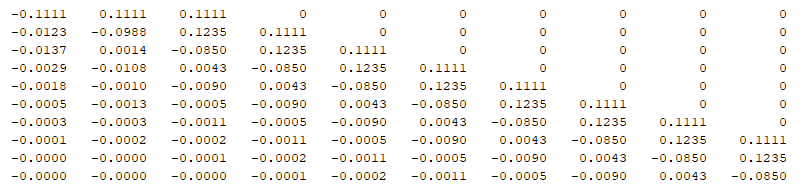
\includegraphics[width=1.1\textwidth]{matrix_images/b1.PNG}
                \caption{Matriz B}
        \end{figure}
    Ahora calculemos el radio espectral de la matriz $B$. Para ello calcularemos los eigenvalores de $B$:
    $$eig(B)=\begin{bmatrix}
    -0.0214 + 0.0911i\\
  -0.0214 - 0.0911i\\
  -0.0586 + 0.0764i\\
  -0.0586 - 0.0764i\\
  -0.0937 + 0.0417i\\
  -0.0937 - 0.0417i\\
  -0.1441 + 0.0167i\\
  -0.1441 - 0.0167i\\
  -0.1436 + 0.0000i\\
  -0.1111 + 0.0000i\\
    \end{bmatrix}
    $$
    El radio espectral de $B$ es el mayor eigenvalor en valor absoluto de $B$.
    $$\rho (B) = 0.1450 <1$$
    Por lo que concluimos que el método CONVERGE.
    
    \item $Dx^{k+1}=-(M+N)x^k + b$ 
    \begin{itemize}
        \item Despejamos para obtener B:
        $$x^{k+1}=-D^{-1}(M+N)x^k + D^{-1}b$$ 
        $$B=-D^{-1}(M+N)$$
    \item Calculamos la matriz B:
    \begin{figure}[H]
                \centering
                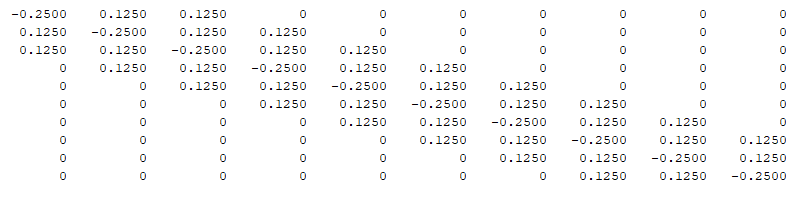
\includegraphics[width=1.1\textwidth]{matrix_images/b2.PNG}
                \caption{Matriz B}
        \end{figure}
    \item Calculamos el radio espectral de $B$:
     Para ello calcularemos los eigenvalores de $B$:
    $$eig(B)=\begin{bmatrix}
              -0.5000\\
           -0.5000\\
           -0.4222\\
           -0.4096\\
           -0.3327\\
           -0.2842\\
           -0.2500\\
           -0.0874\\
            0.0814\\
            0.2048\\
    \end{bmatrix}
    $$
    El radio espectral de $B$ es el mayor eigenvalor en valor absoluto de $B$.
    $$\rho (B) = 0.5000<1$$
    \item Entonces concluimos que el método CONVERGE.
    \end{itemize}
    
    
    
    
    \item $(M+N)x^{k+1}=-Dx^k + b$
    \begin{itemize}
        \item Despejamos para obtener B:
        $$x^{k+1}=-(M+N)^{-1}Dx^k + b$$ 
        $$B=-(M+N)^{-1}D$$
    \item Calculamos la matriz B:
    \begin{figure}[H]
                \centering
                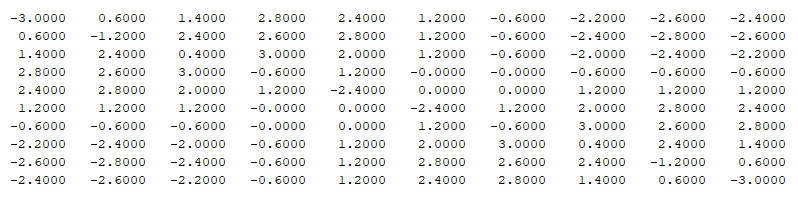
\includegraphics[width=1.1\textwidth]{matrix_images/b3.PNG}
                \caption{Matriz B}
        \end{figure}
    \item Calculamos el radio espectral de $B$:
    Para ello calcularemos los eigenvalores de $B$:
    $$eig(B)=\begin{bmatrix}
            -11.4356\\
           -4.0000\\
           -3.5182\\
           -3.0054\\
           -2.4411\\
           -2.3688\\
           -2.0000\\
           -2.0000\\
            4.8821\\
   12.2870
    \end{bmatrix}
    $$
    El radio espectral de $B$ es el mayor eigenvalor en valor absoluto de $B$.
    $$\rho (B) = 12.2870>1$$
    \item Entonces concluimos que el metodo NO CONVERGE.
    \end{itemize}
\end{itemize} 

% Ejercicio 5
\subsection{Ejercicio 5}
Derivar el sistema lineal usando la aproximación de Diferencias Finitas en la ecuación diferencial parcial elíptica:
\begin{center}
  $ \frac{\partial^2 T}{\partial x^2} + \frac{\partial^2 T}{\partial y^2} = f(x,y)$    
\end{center}

El paso de las diferencias son: $ \Delta x = \Delta y = 0.25 $ y las condiciones de frontera son:
\begin{center}
  $T(x,0) = 1-x$\\
  $T(1,y)=y$\\
  $T(0,y)=1$\\
  $T(x,1)=1$    
\end{center}

\textbf{Solución}:

De los datos, obtenemos los dominios del problema [0, 1].

Entonces haciendo diferencias finitas tenemos:
\begin{center}
  $ \frac{\partial^2 T(x_i , y_i)}{\partial x^2} = \frac{T_{i+1,j} - 2 T_{i,j} + T_{i-1,j}}{\Delta x ^2}$\\
  $ \frac{\partial^2 T(x_i , y_i)}{\partial y^2} = \frac{T_{i,j+1} - 2 T_{i,j} + T_{i,j-1}}{\Delta y ^2}$\\
\end{center}

Entonces, por aproximación tenemos que:
\begin{center}
  $f(x,y) = \frac{T_{i+1,j} - 2 T_{i,j} + T_{i-1,j}}{\Delta x ^2} + \frac{T_{i,j+1} - 2 T_{i,j} + T_{i,j-1}}{\Delta y ^2}$\\
  $f(x,y) = \frac{T_{i+1,j} + T_{i-1,j} - 4 T_{i,j} + T_{i,j+1} + T_{i,j-1}}{0.25 ^2} $\\
  $f(x,y) = 16*T_{i+1,j} + 16*T_{i-1,j} - 48* T_{i,j} + 16*T_{i,j+1} + 16*T_{i,j-1} $\\
\end{center}

Como el intervalo es de [0,1] con paso de 0.25, tenemos 16 puntos: 0, 0.25, 0.5, 0.75, 1 en X y Y. Generando una malla en dichos intervalos.

De los cuales, faltaría calcular los puntos: (0.25, 0.25), (0.25, 0.5), (0.25, 0.75), (0.5,0.25), (0.5,0.5), (0.5, 0.75), (0.75, 0.25), (0.75, 0.5) y (0.75, 0.75).\\

Los cuales se calculan como:

i=1, j=1(0.25,0.25):\\
$f(x_1,y_1) = 16*T_{2,1} + 16*T_{0,1} - 48 T_{1,1} + 16*T_{1,2} + 16*T_{1,0}$\\

i=1, j=2(0.25,0.5):\\
$f(x_1,y_2) = 16*T_{2,2} + 16*T_{0,2} - 48 T_{1,2} + 16*T_{1,3} + 16*T_{1,1}$\\

i=1, j=3(0.25,0.75):\\
$f(x_1,y_3) = 16*T_{2,3} + 16*T_{0,3} - 48 T_{1,3} + 16*T_{1,4} + 16*T_{1,2}$\\

i=2, j=1(0.5,0.25):\\
$f(x_2,y_1) = 16*T_{3,1} + 16*T_{1,1} - 48 T_{2,1} + 16*T_{2,2} + 16*T_{2,0}$\\

i=2, j=2(0.5,0.5):\\
$f(x_2,y_2) = 16*T_{3,2} + 16*T_{1,2} - 48 T_{2,2} + 16*T_{2,3} + 16*T_{2,1}$\\

i=2, j=3(0.5,0.75):\\
$f(x_2,y_3) = 16*T_{3,3} + 16*T_{1,3} - 48 T_{2,3} + 16*T_{2,4} + 16*T_{2,2}$\\

i=3, j=1(0.5,0.25):\\
$f(x_3,y_1) = 16*T_{4,1} + 16*T_{2,1} - 48 T_{3,1} + 16*T_{3,2} + 16*T_{3,0}$\\

i=3, j=2(0.5,0.5):\\
$f(x_3,y_2) = 16*T_{4,2} + 16*T_{2,2} - 48 T_{3,2} + 16*T_{3,3} + 16*T_{3,1}$\\

i=3, j=3(0.5,0.75):\\
$f(x_3,y_3) = 16*T_{4,3} + 16*T_{2,3} - 48 T_{3,3} + 16*T_{3,4} + 16*T_{3,2}$\\

Calculando los respectivos valores:

$T_{0,1} = T(0, 0.25) = 1 $, $T_{4,1} = T(1,0.25) = 0.25$\\
$T_{0,2} = T(0, 0.5) = 1$, $T_{4,2} = T(1,0.5) = 0.5 $\\
$T_{0,3} = T(0, 0.75) = 1$, $T_{4,3} = T(1,0.75) = 0.75 $\\
$T_{1,0} = T(0.25, 0) = 0.75$, $T_{2,0} = T(0.5, 0) = 0.5$, $T_{3,0} = T(0.75, 0) = 0.25$\\
$T_{1,4} = T(0.25, 1) = 1$, $T_{2,4} = T(0.5,1) = 1$, $T_{3,4} = T(0.75,1) = 1$\\
Solo quedaría calcular los puntos:

$T_{1,1} $, $T_{2,1} $, $T_{3,1} $\\
$T_{1,2}$, $T_{2,2} $, $T_{3,2} $\\
$T_{1,3} $, $T_{2,3} $, $T_{3,3} $\\
Los cuales se obtiene de la solución del sistema de ecuaciones formado arriba, el cual se expresa de la siguiente manera:

$f(x_1,y_1) = 16*T_{2,1} + 16 - 48 T_{1,1} + 16*T_{1,2} + 16*0.25$\\
$f(x_1,y_2) = 16*T_{2,2} + 16 - 48 T_{1,2} + 16*T_{1,3} + 16*T_{1,1}$\\
$f(x_1,y_3) = 16*T_{2,3} + 16 - 48 T_{1,3} + 16 + 16*T_{1,2}$\\
$f(x_2,y_1) = 16*T_{3,1} + 16*T_{1,1} - 48 T_{2,1} + 16*T_{2,2} + 16*0.5$\\
$f(x_2,y_2) = 16*T_{3,2} + 16*T_{1,2} - 48 T_{2,2} + 16*T_{2,3} + 16*T_{2,1}$\\
$f(x_2,y_3) = 16*T_{3,3} + 16*T_{1,3} - 48 T_{2,3} + 16 + 16*T_{2,2}$\\
$f(x_1,y_1) = 16*0.25 + 16*T_{2,1} - 48 T_{3,1} + 16*T_{3,2} + 16*0.25$\\
$f(x_2,y_2) = 16*0.5 + 16*T_{2,2} - 48 T_{3,2} + 16*T_{3,3} + 16*T_{3,1}$\\
$f(x_3,y_3) = 16*0.75 + 16*T_{2,3} - 48 T_{3,3} + 16 + 16*T_{3,2}$\\

Dandole una forma de Matrices y vectores tenemos:
\[
\begin{bmatrix}
    -48 & 16 & 0 & 16 & 0 & 0 & 0 & 0\\
    16 & -48 & 16 & 0 & 16 & 0 & 0 & 0 & 0 \\
    0 &  0 & -48 & 16 & 0 & 16 & 0 & 0 & 0 \\
    16 & 0 & 0 & -48 & 16 & 0 & 16 & 0 & 0 \\
    0 & 16 & 0 & 16 & -48 & 16 & 0 & 16 & 0 \\
    0 & 0 & 16 & 0 & 16 & -48 & 0 & 0 & 16  \\
    0 & 0 & 0& 16 & 0 & 0 & -48 & 16 & 0\\
    0 & 0 & 0 & 0 & 16 & 0 & 16 & -48 & 16 \\
    0 & 0 & 0 & 0 & 0 & 16 & 0 & 16 & -48 \\
\end{bmatrix}
+
\begin{bmatrix}
    T_{1,1} \\
    T_{1,2} \\
    T_{1,3} \\
    T_{2,1} \\
    T_{2,2} \\
    T_{2,3} \\
    T_{3,1} \\
    T_{3,2} \\
    T_{3,3} 
\end{bmatrix}
=
\begin{bmatrix}
    f(0.25, 0.25) - 20 \\
    f(0.25, 0.5) - 16\\
    f(0.25, 0.75) - 32\\
    f(0.5, 0.25) - 8\\
    f(0.5, 0.5) \\
    f(0.5, 0.75) - 16\\
    f(0.75, 0.25) -8 \\
    f(0.75, 0.5) - 8 \\
    f(0.75, 0.75) - 28 \\
\end{bmatrix}
\]

Como se puede observar, se generó una matriz pentadiagonal (2 vecinos iguales de la diagonal), para resolver dicha ecuación depende exclusivamente de la función f(x,y). 

% Ejercicio 6
\subsection{Ejercicio 6}
Para resolver el siguiente bloque de sistema lineal:
\[
    \begin{bmatrix}
    A_{1} & B\\
    B & A_{2}
    \end{bmatrix}
    \begin{bmatrix}
    x\\ 
    y 
    \end{bmatrix} = 
    \begin{bmatrix}
    b_{1}\\ 
    b_{2}
    \end{bmatrix}
\]
Considere los siguientes métodos:\\
\begin{itemize}
    \item $ A_{1}x^{(k + 1)} + By^{(k)} =  b_{1}$ , $Bx^{(k)} + A_{2}y^{(k + 1)} =  b_{2}$ 
    \item $ A_{1}x^{(k + 1)} + By^{(k)} =  b_{1}$ , $Bx^{(k + 1)} + A_{2}y^{(k + 1)} =  b_{2}$ 
\end{itemize}

Encontrar las condiciones suficientes de modo que los dos casos sean convergentes para cualquier elección de los datos iniciales de $x^{(0)}$,  $y^{(0)}$\\
Solución: Método (1) es un sistema desacoplado en el desconocido $x^{k+1}$ y $y^{k+1}$. Asumimos que que $A_1$ y $A_2$ son invertibles, método $(1)$ converge si $ \rho (A_1^{-1}B) < 1 $ y $\rho (A_2^{-1}B) < 1 $. en el caso del método $(2)$ tenemos una sistema acoplado para resolver en cada los $x^{k+1}$ y $y^{k+1}$ desconocidos. Resolviendo formalmente la primera ecuación con respecto a $x^{k+1}$  y sustituyendo en la segunda podemos ver que el método $(2)$ es convergente si $\rho (A_2^{-1}BA_1^{-1}B) < 1 $. \\
\textbf{Solución}\\
\begin{itemize}
    \item $ A_{1}x^{(k + 1)} + By^{(k)} =  b_{1}$ , $Bx^{(k)} + A_{2}y^{(k + 1)} =  b_{2}$ 
    \begin{eqnarray*}
        A_{1}x^{(k + 1)} + By^{(k)} =  b_{1} & , & Bx^{(k)} + A_{2}y^{(k + 1)} =  b_{2}\\
        x^{(k + 1)}  =  A_{1}^{-1}b_{1} - A_{1}^{-1}By^{(k)}& , & y^{(k + 1)} =  A_{2}^{-1}b_{2} + A_{2}^{-1}Bx^{(k)}
    \end{eqnarray*} 
    Si 
    \begin{eqnarray*}
        B_{M1} = -A_{1}^{-1}B & , & b_{M1} =  A_{1}^{-1}b\\
        B_{M2} = A_{2}^{-1}B & , & b_{M2} =  A_{2}^{-1}b
    \end{eqnarray*} 
    Entonces
    \begin{eqnarray*}
        x^{(k + 1)} = B_{M1}y^{(k)} + b_{M1} & , & y^{(k + 1)} = B_{M2}y^{(k)} + b_{M2}
    \end{eqnarray*} 
    Para que $x^{(k + 1)}$ converja a $x$:
    \begin{eqnarray*}
        x = B_{M1}y + b_{M1} & , & x^{(k + 1)} = B_{M1}y^{(k)} + b_{M1}\\
        (x - x^{(k + 1)}) & = &  B_{M1}(y - y^{(k)})
    \end{eqnarray*} 
    
    \begin{eqnarray*}
        y = B_{M2}x + b_{M2} & , & y^{(k + 1)} = B_{M2}x^{(k)} + b_{M2}\\
        (y - y^{(k + 1)}) & = &  B_{M2}(x - x^{(k)})
    \end{eqnarray*} 
    
    Asumimos que $k = k - 1$ en $(y - y^{(k + 1)}) = B_{M2}(x - x^{(k)}$, entonces 
     \begin{eqnarray*}
        (y - y^{(k + 1)}) & = &  B_{M2}(x - x^{(k)})\\
        (y - y^{(k)}) & = &  B_{M2}(x - x^{(k - 1)})
    \end{eqnarray*} 
    
    Si reemplazamos $(y - y^{(k)})$ obtenido en $ (x - x^{(k + 1)}) = B_{M1}(y - y^{(k)})$ obtenemos lo siguiente:
    
    \begin{eqnarray*}
        (x - x^{(k + 1)}) & = &  B_{M1}\underbrace{(y - y^{(k)})}\\
        (x - x^{(k + 1)}) & = &  B_{M1}(B_{M2}(x - x^{(k - 1)}))\\
        (x - x^{(k + 1)}) & = &  B_{M1}(B_{M2}^{2}(x - x^{(k - 2)}))\\
        (x - x^{(k + 1)}) & = &  B_{M1}(B_{M2}^{3}(x - x^{(k - 3)}))\\
        (x - x^{(k + 1)}) & = &  B_{M1}(B_{M2}^{4}(x - x^{(k - 4)}))\\
        \vdots \\
        (x - x^{(k + 1)}) & = &  B_{M1}(B_{M2}^{k}(x - x^{(k - k)}))\\
        (x - x^{(k + 1)}) & = &  B_{M1}(B_{M2}^{k}(x - x^{(0)}))
    \end{eqnarray*}
    Una condición suficiente para determinar la convergencia de $x^{(k + 1)}$ a $x$ para cualquier valor de $x^{(0)}$ es que $B_{M2}^{k}$ converja. Para que $B_{M2}^{k}$ converja se tiene que cumplir que  $\rho (B_{M2}) < 1  \rightarrow  \rho (A_{2}^{-1}B) < 1$ \\
    
    %Convergencia de y
    Para que $y^{(k + 1)}$ converja a $y$. Se tiene 
    \begin{eqnarray*}
        (x - x^{(k + 1)}) & = &  B_{M1}(y - y^{(k)})
    \end{eqnarray*} 
    y
    \begin{eqnarray*}
        (y - y^{(k + 1)}) & = &  B_{M2}(x - x^{(k)})
    \end{eqnarray*} 
    
    Asumimos que $k = k -1$ en la primera ecuación y luego reemplazamos en la segunda ecuación:
    \begin{eqnarray*}
        (x - x^{(k + 1)}) & = &  B_{M1}(y - y^{(k)})\\
        (x - x^{(k)}) & = &  B_{M1}(y - y^{(k - 1)})
    \end{eqnarray*} 
    Reemplazamos $(x - x^{(k)}) =  B_{M1}(y - y^{(k - 1)})$  en 
     \begin{eqnarray*}
        (y - y^{(k + 1)}) & = &  B_{M2}(x - x^{(k)})\\
        (y - y^{(k + 1)}) & = &  B_{M2}( B_{M1}(y - y^{(k - 1)}))\\
    \end{eqnarray*} 
    Desarrollamos
    \begin{eqnarray*}
        (y - y^{(k + 1)}) & = &  B_{M2} B_{M1}(y - y^{(k - 1)})\\
        (y - y^{(k + 1)}) & = &  B_{M2} B_{M1}^{2}(y - y^{(k - 2)})\\
        (y - y^{(k + 1)}) & = &  B_{M2} B_{M1}^{3}(y - y^{(k - 3)})\\
        (y - y^{(k + 1)}) & = &  B_{M2} B_{M1}^{4}(y - y^{(k - 4)})\\
        \vdots \\
        (y - y^{(k + 1)}) & = &  B_{M2} B_{M1}^{k}(y - y^{(k - K)})\\
        (y - y^{(k + 1)}) & = &  B_{M2} B_{M1}^{k}(y - y^{(0)})
    \end{eqnarray*} 
    
    
    Una condición suficiente para determinar la convergencia de $y^{(k + 1)}$ a $y$ para cualquier valor de $y^{(0)}$ es que $B_{M1}^{k}$ converja. Para que $B_{M1}^{k}$ converja se tiene que cumplir que  $\rho (B_{M1}) < 1 \rho (A_{1}^{-1}B) < 1$ \\
    
   
\end{itemize} 

% Ejercicio 7
\subsection{Ejercicio 7}
Considere el sistema lineal $Ax=b$ con:\\\\
\begin{center}
A = 
\[
\begin{bmatrix}
    62 & 24 &  1 &  8 & 15 \\
    23 & 50 &  7 & 14 & 16 \\
     4 &  6 & 58 & 20 & 22 \\
    10 & 12 & 19 & 66 &  3 \\
    11 & 18 & 25 &  2 & 54
\end{bmatrix}
, b = 
\begin{bmatrix}
    110 \\
    110 \\
    110 \\
    110 \\
    110
\end{bmatrix}
\]
\end{center}

\begin{itemize}

\item \textbf{Verificar si los métodos de Jacobi y Gauss-Seidel pueden ser aplicados para resolver el sistema.}\\
Como A no es diagonal dominante o simétrica definida positiva, entonces es necesario calcular el radio espectral de las matrices de iteracion de Jacobi y Gauss-Seidel:

\begin{align}
    B_j  &= -D^{-1}(L+U)  \Rightarrow \rho(B_j) &= 0.9280 \\
    B_gs &= -(D+L)^{-1}U  \Rightarrow \rho(B_gs)&= 0.3066
\end{align}~\\
Como ambos radios espectrales son menores a $1$, entonces el sistema converge con ambos métodos.

\item \textbf{Verificar si el método estacionario de Richardson con parámetro óptimo puede ser aplicado con $P=I$ y $P=D$, donde $D$ es la parte diagonal de A y calcule los valores de $\alpha_{opt}$ y  $\phi_{opt}$.}\\
\begin{align}
    R_p = I - P^{-1}A \Rightarrow R_{(\alpha_k)} = I - \alpha_k P^{-1}A
\end{align}
Para el método estacionario de Richardson:
\begin{align}
(\alpha_k = \alpha) \Rightarrow R_{\alpha} = I - \alpha P^{-1} A  
\end{align}
La iteración $k+1$ del sistema tiene la siguiente forma.
\begin{align}
    x^{k+1} &= x^k + \alpha P^{-1} r^k
\end{align}
Sabiendo que $\alpha_{opt} = \frac{2}{\lambda_1 + \lambda_n}$ y $P^{-1}A$ tiene autovalores reales positivos, es decir:
\begin{align}
    \lambda_1 \geq \lambda_2 \geq \dots \geq \lambda_0 \geq 0
\end{align}
Luego, el sistema converge si y solo si $0 < \alpha < \lambda_1$ y el radio espectral de la matriz iterativa $R_{\alpha}$ es el mínimo si $\alpha = \alpha_{opt}$ con:
\begin{align}
    \rho_{opt} &= min(\rho_{R_{\alpha}}) = \frac{\lambda_1 - \lambda_n}{\lambda_1 + \lambda_n}
\end{align}~\\\\
Caso 1: $P = I$\\\\
\begin{align}
    P^{-1}A = I^{-1}A = A \Rightarrow \lambda(A) &= \{110;66.2;58.1;31.8;23.7\} \\
    \alpha_{opt} &= 0.00149 \\
    \rho_{opt} &= 0.6452
\end{align}
Los autovalores de A son reales positivos y $\phi_{opt} < 1$, por lo que el método puede ser aplicado.\\\\

Caso 2: $P = D$\\\\
\begin{align}
    P^{-1}A = D^{-1}A \Rightarrow \lambda(D^{-1}A) &= \{1.92;1.12;0.95;0.577;0.422\} \\
    \alpha_{opt} &= 0.8510 \\
    \rho_{opt} &= 0.0.6407
\end{align}
Los autovalores de A son reales positivos y $\phi_{opt} < 1$, por lo que el método puede ser aplicado.

\end{itemize} 

% Ejercicio 8
\subsection{Ejercicio 8}
Considere el sistema Ax = b:
\[
\begin{bmatrix}
    5 & 7 & 6 & 5\\
    7 & 10 & 8 & 7 \\
    6 &  8 & 10 & 9 \\
    5 & 7 & 9 & 10\\
\end{bmatrix}
\begin{bmatrix}
    x_{1} \\
    x_{2} \\
    x_{3} \\
    x_{4} \\
\end{bmatrix}
=
\begin{bmatrix}
    22 \\
    32\\
    33\\
    31\\
\end{bmatrix}
\]

Analizar las propiedades de convergencia de los métodos de Jacobi y Gauss-Seidel aplicado al sistema de arriba en sus formas de punto y bloque (para un bloque de 2 × 2 partición de A).

\textbf{Solución}:

Haciendo el método de Jacobi por bloques, tenemos:
\begin{center}
$X^{k+1}_i = A^{-1}_{ii}  (B_i − \sum_{j=1, j \neq i}^{n} A_{ij} X^k _ j)$
\end{center}

Haciendo el método de Gauss-Seidel por bloques, tenemos:
\begin{center}
$X^{k+1}_i = A^{-1}_{ii}  (B_i − \sum_{j=1}^{i-1} A_{ij} X^{k+1} _ j − \sum_{j=i+1}^{n} A_{ij} X^{k} _ j )$
\end{center}

Sabemos que la convergencia (por bloques) se sigue manteniendo, y que se analiza la convergencia de ambos métodos según la descomposición y pre condicionamiento aplicado al sistema.

\textbf{Gauss Seidel}

En el caso de Gauss Seidel, tenemos:
$x^{(k+1)}={-(L+D)}^{-1}{U}x^{(k)}+{(L+D)}^{-1}b$

Donde D es la diagonal de A, L es el triangulo inferior a la diagonal de A y U es el triangulo superior de A.

Tal que: L + D + U = A

La convergencia se analiza según el radio espectral de la matriz M, definida por:

$x^{(k+1)}=Mx + c$, donde $M=-(L+D)^{-1} U$ y $c=(L+D)^{-1} b$.

Teniendo A y b como datos, calculamos M:
\begin{center}
\[
\begin{bmatrix}
    0 & -1.4 & -1.2 & -1 \\
    0 & 0.98 & 0.04 & 0 \\
    0 &  0.056 & 0.688 & -0.3 \\
    0 & -0.0364 & -0.0472 & 0.77 \\
\end{bmatrix}
\]    
\end{center}

Calculamos su radio espectral (máximo de los valores absolutos de la matriz M menores a 1).

$\lambda_1 =0$, $\lambda_2 = 0.99690$, $\lambda_3 = 0.83728$ , $\lambda_4 = 0.60382$.

El radio espectral de Gauss Seidel para este sistema es:
\begin{center}
    $\rho_gs (M) = 0.99690 < 1$
\end{center}

Vemos que si converge.

\textbf{Jacobi}

En el caso de Jacobi, tenemos:
$x^{(k+1)}={-(D)}^{-1}{R}x^{(k)}+{(D)}^{-1}b$

Donde D es la diagonal de A, R es la matriz A menos la diagonal.

Tal que: D + R = A

La convergencia se analiza según el radio espectral de la matriz M, definida por:

$x^{(k+1)}=Mx + c$, donde $M=-(D)^{-1} R$ y $c=(D)^{-1} b$.

Teniendo A y b como datos, calculamos M:
\begin{center}
\[
\begin{bmatrix}
    0 & -1.4 & -1.2 & -1 \\
    -0.7 & 0 & -0.8 & -0.7 \\
    -0.6 &  -0.8 & 0 & -0.9 \\
    -0.5 & -0.7 & -0.9 & 0 \\
\end{bmatrix}
\]    
\end{center}

Calculamos su radio espectral (máximo de los valores absolutos de la matriz M menores a 1).

$\lambda_1 = -2.47579$, $\lambda_2 = 0.56220$, $\lambda_3 = 0.99845$ , $\lambda_4 = 0.91514$.

El radio espectral de Gauss Seidel para este sistema es:
\begin{center}
    $\rho_j (M) = 0.99845 < 1$
\end{center}

Vemos que si converge.

Y comparando los radios espectrales, tenemos que:

\begin{center}
    $\rho_j ^ 2 (M) = \rho_{gs} (M) = 0.99690 < 1$
\end{center}

Por lo tanto, Ambos métodos convergen y el más rápido es el Jacobi por bloques. 

% Ejercicio 11
\subsection{Ejercicio 11}
%==============================================================================================================
%==============================================================================================================
% Para el grupo de Jefferson
%==============================================================================================================
%==============================================================================================================

Considerando el sistema lineal
$$ Ax=b$$
$$ A=\begin{pmatrix}
     3 &  2 \\
     2 &  6 \\
    \end{pmatrix}\ $$
    
$$ b=\begin{pmatrix}
     2 \\
     -8 \\
    \end{pmatrix}\ $$
    
Escribe la función $ \Phi(x) $ y muestre una interpretación gráfica de la solución de dicho sistema lineal. Pruebe algunas iteraciones del Método del Gradiente después de probar su convergencia.\\

\textbf{Solución:}

El Método del Gradiente converge para el caso debido a que es una matriz simétrica positiva. Esto es porque sus autovalores son positivos ($ \lambda _1 = 2$, $\lambda _2 = 7$).

Considerando un valor inicial 
$$x_0 = \begin{pmatrix}
     15 \\
     -13 \\
    \end{pmatrix}\ $$
Podemos mostrar en la siguiente tabla los valores del los vectores en cada iteración

\begin{table}[h]
    \centering
    \begin{tabular}{r|l|l}
        Iteración & $x$ &    $y$   \\
        \hline
         0  &  15  &  -13 \\
         1  &  10.8548 & -3.2465 \\
         2  &  5.9412 & -5.3348 \\
         3  &  4.6845 & -2.3779 \\
         4  &  3.1948 & -3.0110 \\
         5  &  2.8138 & -2.1146 \\
         6  &  2.3622 & -2.3065 \\
         7  &  2.2467 & -2.0347 \\
         8  &  2.1098 & -2.0929 \\
         9  &  2.0748 & -2.0105 \\
         10  & 2.0333  & -2.0282 \\
         11  & 2.0227  & -2.0032 \\
         12  & 2.0101  & -2.0085 \\
         13  & 2.0069  & -2.0010 \\
         14  & 2.0031  & -2.0026 \\
    \end{tabular}
\end{table}

\begin{center}
    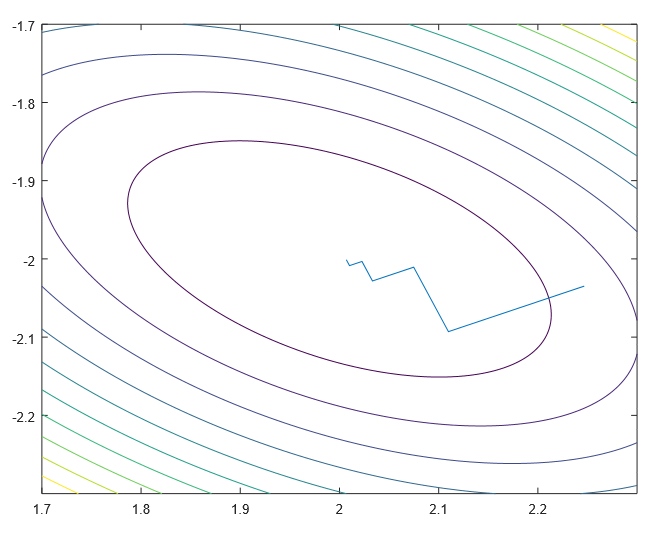
\includegraphics[scale=0.5]{AlfioQuarteroni/Jefferson.png} 
\end{center}

De acuerdo a la gráfica, el Método del Gradiente converge a la solución que está en $(2,-2)$ y es el mínimos de la función cuadrática $\Phi(x)$\\

%==============================================================================================================
%==============================================================================================================
% Para el grupo de Victor
%==============================================================================================================
%==============================================================================================================

Considerando el sistema lineal
$$ Ax=b$$
$$ A=\begin{pmatrix}
     3 &  2 \\
     2 &  6 \\
    \end{pmatrix}\ $$
    
$$ b=\begin{pmatrix}
     2 \\
     -8 \\
    \end{pmatrix}\ $$
    
Escribe la función $ \Phi(x) $ y muestre una interpretación gráfica de la solución de dicho sistema lineal. Pruebe algunas iteraciones del Método del Gradiente después de probar su convergencia.\\

\textbf{Solución:}

El Método del Gradiente converge para el caso debido a que es una matriz simétrica positiva. Esto es porque sus autovalores son positivos ($ \lambda_1=2, \lambda_2=7$).

Considerando un valor inicial 
$$x_0 = \begin{pmatrix}
     15 \\
     -13 \\
    \end{pmatrix}\ $$
Podemos mostrar en la siguiente tabla los valores del los vectores en cada iteración

\begin{table}[h]
    \centering
    \begin{tabular}{r|l|l}
        Iteración & $x$ &    $y$   \\
        \hline
         0  &  -9  &  8 \\
         1  & -6.08562 & -0.51897 \\
         2  &  -1.39448 & 1.08589 \\
         3  & -0.49513 & -1.54297 \\
         4  & 0.95250 & -1.04773 \\
         5  &   1.23003 & -1.85897 \\
         6  & 1.67675 &  -1.70614 \\
         7  & 1.76240 & -1.95648 \\
         8  & 1.90025 & -1.90932 \\
         9  & 1.92668 & -1.98657 \\
         10  & 1.96922 & -1.97202\\
         11  & 1.97737 & -1.99586 \\
         12  & 1.99050 & -1.99136 \\
         13  & 1.99302 & -1.99872 \\
         14  & 1.99707 & -1.99734 \\
    \end{tabular}
\end{table}

\begin{center}
    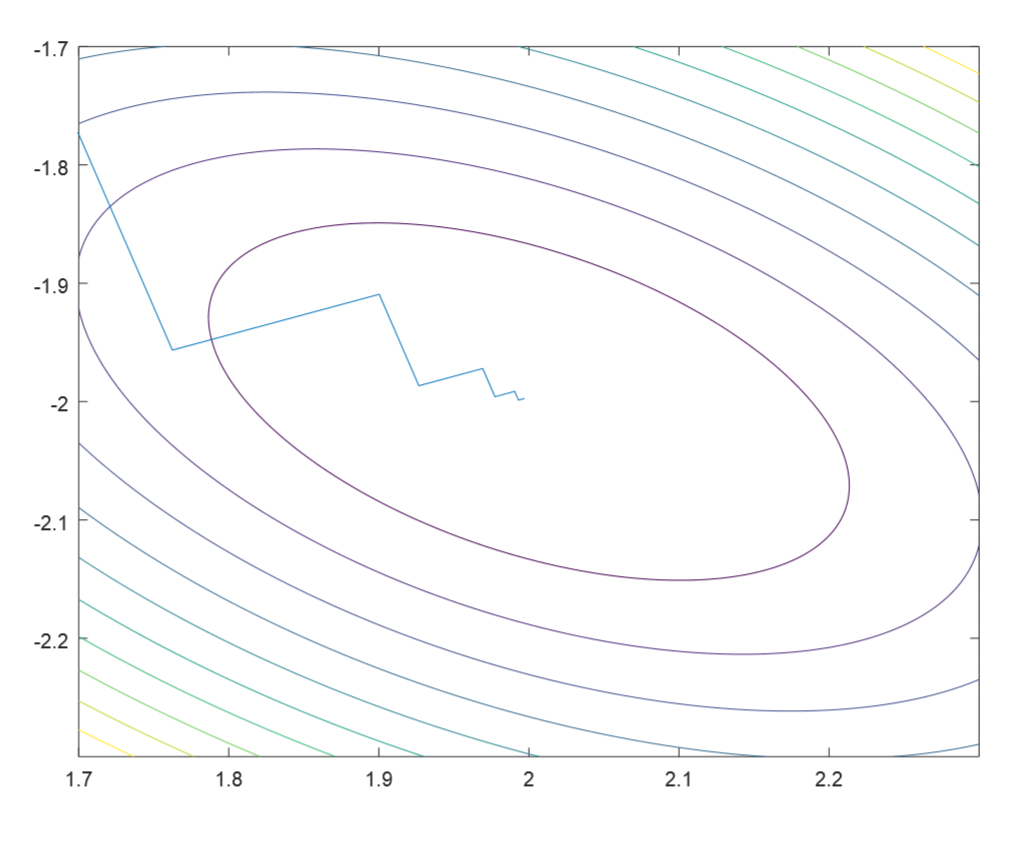
\includegraphics[scale=0.5]{AlfioQuarteroni/Victor.png} 
\end{center}


De acuerdo a la gráfica, el Método del Gradiente converge a la solución que está en $(2,-2)$ y es el mínimos de la función cuadrática $\Phi(x)$\\
%==============================================================================================================
%==============================================================================================================
% Para el grupo de Vittorino
%==============================================================================================================
%==============================================================================================================

Considerando el sistema lineal
$$ Ax=b$$
$$ A=\begin{pmatrix}
     3 &  2 \\
     2 &  6 \\
    \end{pmatrix}\ $$
    
$$ b=\begin{pmatrix}
     2 \\
     -8 \\
    \end{pmatrix}\ $$
    
Escribe la función $ \Phi(x) $ y muestre una interpretación gráfica de la solución de dicho sistema lineal. Pruebe algunas iteraciones del Método del Gradiente después de probar su convergencia.\\

\textbf{Solución:}

El Método del Gradiente converge para el caso debido a que es una matriz simétrica positiva. Esto es porque sus autovalores son positivos ($ \lambda_1=2, \lambda_2=7$).

Considerando un valor inicial 
$$x_0 = \begin{pmatrix}
     15 \\
     -13 \\
    \end{pmatrix}\ $$
Podemos mostrar en la siguiente tabla los valores del los vectores en cada iteración

\begin{table}[h]
    \centering
    \begin{tabular}{|r|l|l|}
        Iteración & $x$ &    $y$   \\
        \hline
         0  &  11  & 4  \\
         1  & 5.3233 & -3.8601 \\
         2  & 2.3889 & -1.7407 \\
         3  & 2.1436 & -2.0804 \\
         4  & 2.0168 & -1.9888 \\
         5  & 2.0062 & -2.0035 \\
         6  & 2.0007 & -1.9995 \\
         7  & 2.0003 & -2.0002\\

    \end{tabular}
\end{table}

\begin{center}
    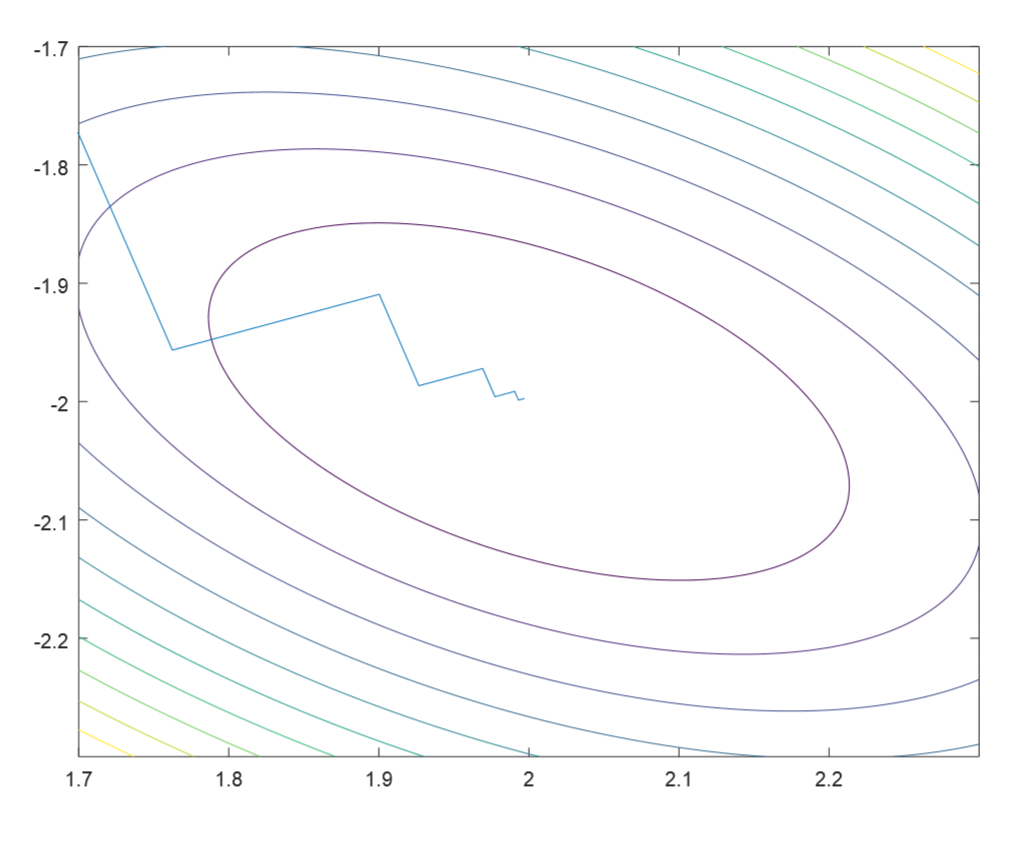
\includegraphics[scale=0.5]{AlfioQuarteroni/Victor.png} 
\end{center}

De acuerdo a la gráfica, el Método del Gradiente converge a la solución que está en $(2,-2)$ y es el mínimos de la función cuadrática $\Phi(x)$\\

%==============================================================================================================
%==============================================================================================================
% Para el grupo de Laura
%==============================================================================================================
%==============================================================================================================

Considerando el sistema lineal
$$ Ax=b$$
$$ A=\begin{pmatrix}
     3 &  2 \\
     2 &  6 \\
    \end{pmatrix}\ $$
    
$$ b=\begin{pmatrix}
     2 \\
     -8 \\
    \end{pmatrix}\ $$
    
Escribe la función $ \Phi(x) $ y muestre una interpretación gráfica de la solución de dicho sistema lineal. Pruebe algunas iteraciones del Método del Gradiente después de probar su convergencia.\\

\textbf{Solución:}

El Método del Gradiente converge para el caso debido a que es una matriz simétrica positiva. Esto es porque sus autovalores son positivos ($ \lambda_1=2, \lambda_2=7$).

Considerando un valor inicial 
$$x_0 = \begin{pmatrix}
     15 \\
     -13 \\
    \end{pmatrix}\ $$
Podemos mostrar en la siguiente tabla los valores del los vectores en cada iteración

\begin{table}[h]
    \centering
    \begin{tabular}{|r|l|l|}
        Iteración & $x$ &    $y$   \\
        \hline
         0  &  -11  &  -9 \\
         1  & -3.2124 & 0.99158 \\
         2  & 1.1873 & -2.43762 \\
         3  & 1.6741 & -1.81298 \\
         4  & 1.9492 & -2.02736 \\
         5  & 1.9796 & -1.98831 \\
         6  & 1.9968 & -2.00171 \\
         7  & 1.9987 & -1.99927\\
    \end{tabular}
\end{table}

\begin{center}
    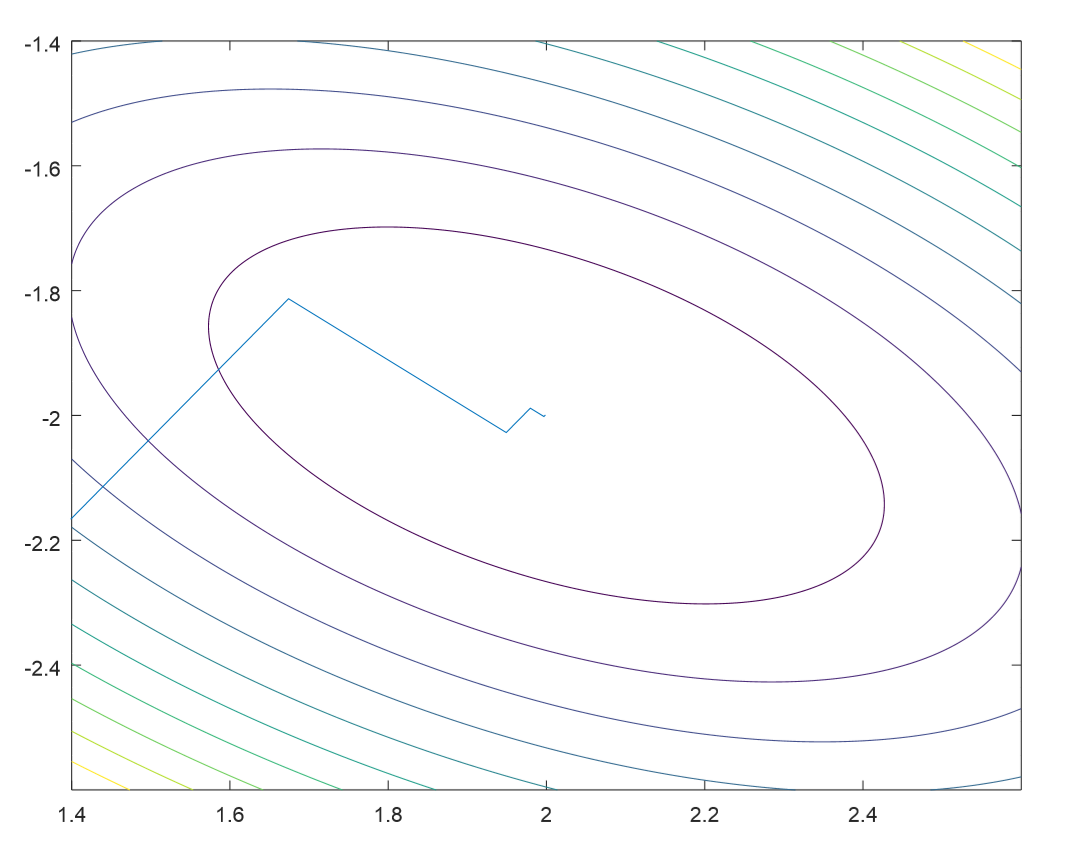
\includegraphics[scale=0.5]{AlfioQuarteroni/Laura.png} 
\end{center} 

De acuerdo a la gráfica, el Método del Gradiente converge a la solución que está en $(2,-2)$ y es el mínimos de la función cuadrática $\Phi(x)$\\ 

% Ejercicio 13
\subsection{Ejercicio 13}
Muestre que el coeficiente $\alpha_k$  y $\beta_k$ en el método de la gradiente conjugada puede ser escrita en la forma alternativa:

\[\alpha_k=\frac{||r^{(K)}||_2^2}{{p^{(k)}}^T}Ap^{(k)} , \beta_k=\frac{||r^{(k+1)}||_2^2}{||r^{(k)}||_2^2} \]

\textbf{Solución}\\
Para $\alpha_k=\frac{||r^{(K)}||_2^2}{{p^{(k)}}^T}Ap^{(k)}$\\
Se sabe que: $r^{k+1} = r^k - \alpha_k AP^{k} $ , por lo que:\\
\[AP^k = \frac{r^k - r^{k+1}}{\alpha_k} ....(I)\]
\[(r^k)^T AP^k = \frac{(r^k)^T r^k - (r^k)^T r^{k+1}}{\alpha_k}\]
Como $(r^k)^T r^{k+1}$ es el producto interno, entonces $(r^k)^T r^{k+1}=0$
\[(r^k)^T AP^k = || r^k ||_2^2 ...(II)\]
\[p^{k+1} = r^{k+1} - \beta_k P\]
\[(P^k)^T AP^k = (r^k - \beta_{k-1})P^{k-1} AP^k\]
\[(P^k)^T AP^k = ((r^k)^T - \beta_{k-1})(P^{k-1})^T)AP^k\]
\[(P^k)^T AP^k = (r^k)^T AP^k - \beta_{k-1}(P^{k-1} AP^k) , (P^{k-1})^T P^T = 0\]
\[(P^k)^T AP^k = (r^k)^T AP^k ...(III)\]
De II y III se tiene que:\\
\[(P^k)^T AP^k = \frac{||r^k||_2^2}{\alpha_k}\]
\[\alpha_k = \frac{||r^k||_2^2}{(P^k) AP^k}\]

Para $\beta_k=\frac{||r^{(k+1)}||_2^2}{||r^{(k)}||_2^2} $\\
Partimos de I se tiene que:
\[(AP^k)^T = \frac{r^k - r^{k+1}}{\alpha_k} r^{k+1}\]
Despejando el producto interno:
\[(AP^k)^T r^{k+1} = \frac{||r^{k+1}||_2^2}{\alpha_k}  ...(IV)\]
Por definición se tiene:
\[\beta_k = \frac{(AP^k)^T r^{k+1}}{(AP^k)^T P^{k+1}}\]
Y del resultado de $\alpha_k=\frac{||r^{(K)}||_2^2}{{p^{(k)}}^T}Ap^{(k)}$ y de IV se tiene:
\[\beta_k = \frac{-\frac{||r^{k+1}||_2^2}{\alpha_k}}{-\frac{||r^k||_2^2}{\alpha_k}}\]
\[\beta_k = \frac{|| r^{k+1} ||_2^2}{||r^k||_2^2}\]
 

% Ejercicio 14
\subsection{Ejercicio 14}
\textbf{Probar que:\\}
    
    \[
        A = \begin{bmatrix}
            4 & -1 & -1 & 0\\
            -1 & 4 & 0 & -1\\
            -1 & 0 & 4 & -1\\
            0 & -1 & -1 & 4\\
        \end{bmatrix}
    \]
    
    es positiva definida con y sin encontrar la factorización de \textit{Cholesky}.\\\\
    
    \textbf{Solución}\\
    
    \textbf{Sin usar Cholesky:}\\
    
    Para que una matriz sea definida positiva, tenemos que probar dos cosas: que sea simétrica y que sus autovalores sean positivos. Como se puede ver, la matriz $A$ es simétrica y sus autovalores son: $\lambda_1 = 2, \lambda_2 = 4, \lambda_3 = 4, \lambda_4 = 6$, todos sus valores positivos. Luego podemos decir que la matriz es positiva definida.\\
        
    \textbf{Cholesky}\\
    
    Debemos encontrar una matriz $H$ tal que $A = H H^T$.
    Para encontrar la matriz usamos las siguientes formulas:
        
        \begin{equation*}
            \begin{split}
                l_{kk} = \sqrt{a_{kk} - \sum_{j=1}^{k-1} l_{kj} ^ 2}\\
                l_{ki} = \frac{a_{ki} - \sum_{j=1}^{i-1} l_{ij} l_{kj} }{l_{ii}}
            \end{split}
        \end{equation*}
        
        Luego la matriz $H$ será:
        
        \[
        H = \begin{bmatrix}
            2 & 0 & 0 & 0\\
            -0.5 & 1.936492 & 0 & 0\\
            -0.5 & -0.129099 & 1.932184 & 0 \\
            0 & -0.516398 & -0.552052 & 1.85164\\
        \end{bmatrix}
       \]
    
    Si multiplicamos $H$ con $H^T$ obtenemos $A$.
 
    \textbf{Resolver el sistema}
    
    \[
        Ax = \begin{bmatrix}
            2\\
            2\\
            2\\
            2\\
        \end{bmatrix}
    \]
    \\\\
    
    \textbf{Solución}\\
    
    Usando $H$ del punto (b), tenemos que:
    \[
        \begin{bmatrix}
            2 & 0 & 0 & 0\\
            -0.5 & 1.936492 & 0 & 0\\
            -0.5 & -0.129099 & 1.932184 & 0 \\
            0 & -0.516398 & -0.552052 & 1.85164\\
        \end{bmatrix} * 
        \begin{bmatrix}
            y_1\\ y_2\\ y_3\\ y_4\\
        \end{bmatrix} = 
        \begin{bmatrix}
            2 \\ 2 \\ 2 \\ 2 \\
        \end{bmatrix}
    \]
    
    Luego:
    $$
    y_1 = 1, \quad y_2 \approx 1.2909942, \quad y_3 \approx 1.380130497, \quad y_4 \approx 1.85163997
    $$
    
    Multiplicando ahora $H^T x^T = y$
    
    \[
        \begin{bmatrix}
            2 & -0.5 & -0.5 & 0\\
            0 & 1.936492 & -0.129099 & -0.516398\\
            0 & 0 & 1.932184 & -0.552052 \\
            0 & 0 & 0 & 1.85164\\
        \end{bmatrix} * 
        \begin{bmatrix}
            x_1\\ x_2\\ x_3\\ x_4\\
        \end{bmatrix} = 
        \begin{bmatrix}
            1 \\ 1.2909942 \\ 1.380130497 \\ 1.85163997 \\
        \end{bmatrix}
    \]
    
    Finalmente tenemos que:
    
    $$
    x_1 = 1, \quad x_2 = 1, \quad x_3 = 1, \quad x_4 = 1
    $$ 


%=========================================================
% James Schott
%=========================================================
\section{James  R.  Schott}

% Ejercicio 8.79
\subsection{Ejercicio 8.79}
Se ha visto en el Teorema 8.41 que $\rho(A)$ es un valor singular de $A$ si $A$ es positiva. En este ejercicio, se usará la extensión de este resultado que dice que $\rho(A)$ es un valor singular de $A$ si $A$ es no negativa. Para los siguientes enunciados asuma que $A$ es una matriz no negativa de $m$ x $m$.

\begin{itemize}
    \item Muestre que $\rho(I_m + A) = 1 + \rho(A)$
    
    \item Muestre que si $ A^k > (0) $ para algún entero positivo $k$, entonces $\rho(A)$ es un simple valor singular de $A$
    
    \item Aplique b) en la matriz $(I_m + A)$ para probar el Teorema 8.49; esto es, probar que para cualquier matriz no negativa irreducible $A$, $\rho(A)$ debe ser un simple valor singular.
\end{itemize}


\textbf{Solución:}

\begin{itemize}

\item Muestre que $\rho(I_m + A) = 1 + \rho(A)$\\
    
    Partimos de la ecuación que nos permite obtener los autovalores de una matriz. Denominaremos $\lambda_1$ a los autovalores de esta matriz.
    
    \begin{equation*}
        det(A - \lambda_1 I) = 0
    \end{equation*}
    
    Definimos una segunda matriz $B = A + I$, y denominaremos a sus autovalores como $\lambda_2$. 
    
    %\[  
        $$det(B - \lambda_2 I) = 0$$
        $$det(A + I - \lambda_2 I) = 0 $$
        $$det(A - I ( \lambda_2 - 1) = 0 $$
    %\]
    
    Si igualamos ambas expresiones, se tiene que:
 
    $$\lambda_1 = \lambda_2 - 1$$
    
    Suponiendo que ambos $\lambda$ ($\lambda_1$ y $\lambda_2$) representan los radios espectrales de las matrices $ A $ y $ I_m + A $ respectivamente, se concluye que:
    
    $$\rho(A) = \rho(I_m + A) - 1$$
    
\item Muestre que si $ A^k > (0) $ para algún entero positivo $k$, entonces $\rho(A)$ es un simple valor singular de $A$\\
    
    Primero, partiendo del presente enunciado, que indica que $ A^k > (0) $, se puede concluir que la matriz $A$ es positiva, ya que para que una potencia de la matriz $A$ sea positiva, cada componente de la matriz $A$ debió ser positivo y diferente de cero. Por lo tanto, la matriz $A$ no solo es no negativa (como lo indica el enunciado general), sino que es positiva.
    
    Segundo, existe un Teorema llamado el Teorema de Perron, que demuestra mediante la relación que existe entre los autovalores y autovectores de una matriz positiva que, el radio espectral de una matriz positiva siempre tiene multiplicidad algebraica de 1, es decir, que existe . Por lo tanto, se puede concluir que $\rho (A)$ es un autovalor simple.
    
\item 

\end{itemize} 

% Ejercicio 8.80
\subsection{Ejercicio 8.80}
Considera cadena homogénea de \textit{Markov} que tiene 3 estados y la matriz
    de transición de transición dado por:
    \[
        P =
            \begin{bmatrix}
                0.50 & 0.25 & 0 \\
                0.50 & 0.50 & 0.25\\
                0 & 0.25 & 0.75
            \end{bmatrix}
    \]
    \begin{itemize}
        \item Mostrar que \textit{P} es primitiva.

        Una matriz $mxm$ no negativa $A$ se dice que es primitiva si existe un $k$, tal que
        $A^k > 0$, esto es, $a_{ij} > 0$ $\forall$ $i$ $\&$ $j$. 
        Para $k = 2$:\\
        \[
            P =
                \begin{bmatrix}
                    0.375 & 0.25 & 0.0625 \\
                    0.50 & 0.4375 & 0.3125\\
                    0.125 & 0.3125 & 0.625
                \end{bmatrix}
        \]
        Ya que la matriz es P es no negativa, además existe un $k = 2$ tal que $P^* = P^2$: $p^*_{ij} > 0$ $\forall$ $i$ $\&$ $j$, por tanto la matriz $P$ es primitiva
        \item Determina la distribución de equilibrio, esto es, encuentra el vector
        $\pi$ tal que $\lim_{t \to \infty} p^{(t)} = \pi$\\\\
        En general:
        \[
            p^{(t)} = P^tp^{(0)} 
        \]
        Ya que $p^{(t)} = P^{(t)}p^{(0)}$, también puede ser expresado como:
        \[
            p^{(t)} = Pp^{(t-1)}
        \]
        El sistema apunta al punto de equilibrio en donde las proporsiones para los estados
        estan dados por las componentes de $\pi$ y esta proporsion no cambia con el tiempo.
        Esto es: $p^{(t)} = p^{(t-1)}$, por tanto:
        \[
                \pi = P\pi  \quad \dots \quad(1)
        \]
        Además ya que este punto representa la probabilidad de un conjunto, la suma de este es igual a 1.
        Esto es:
        \[
                \pi'1_m = 1 \quad \dots \quad(2)
        \]

        Hallando el autovalor $\pi$ a partir de la ecuación $(1)$:
        \[
            \pi = 
                \begin{bmatrix}
                    1 \\
                    2\\
                    2
                \end{bmatrix}
        \]
        De la ecuación $(2)$: (Las probabilidades deben sumar 1).
        Esto es:
        \[
            \pi = 
                \begin{bmatrix}
                    0.2 \\
                    0.4\\
                    0.4
                \end{bmatrix}
        \]
    \end{itemize}

%=========================================================
% Ejercicios Adicionales
%=========================================================

\section{Ejercicios Adicionales}

% Ejercicio Adicionales
\subsection{Ejercicio 1}
Dado el sistema $Ax=b$, donde:

$$
    A=\begin{pmatrix}
     1 &  2 & -2 \\
     1 &  1 &  1 \\
     2 &  2 &  1 
    \end{pmatrix},\ 
    b=\begin{pmatrix}
    1\\
    4\\
    5
    \end{pmatrix}
$$

¿Es posible resolver el sistema por los métodos de Gauss-Seidel y Jacobi? en caso de ser factible halle la solución.

\textbf{Solución:}

Para saber si es posible resolver el sistema por los métodos mencionados se debe hallar el radio de convergencia de cada método:

$$
    B_{J}=\begin{pmatrix}
     2 &  -2 & 2 \\
     -1 &  0 &  -1 \\
     -2 &  -2 &  0 
    \end{pmatrix},\ \rho(B_{J}) = 1.0809*10^{-5}
$$

y

$$
    B_{GS}=\begin{pmatrix}
     0 &  -2 & 2 \\
     0 &  -2 &  1 \\
     0 &  -8 &  6 
    \end{pmatrix},\ \rho(B_{GS}) = 4.8284
$$

De donde se observa que solo es posible resolver el sistema usando el método de Jacobi. Entonces:

Siendo:

$$
    b_{J}=D^{-1}b = \begin{pmatrix}
    1\\
    4\\
    5
    \end{pmatrix}
$$

Entonces:

$$
    x^{(0)}=\begin{pmatrix}
    0\\
    0\\
    0
    \end{pmatrix}
$$

$$
    x^{(1)}=\begin{pmatrix}
    -1\\
    -4\\
    -5
    \end{pmatrix}
$$

$$
    x^{(2)}=\begin{pmatrix}
    -3\\
    2\\
    5
    \end{pmatrix}
$$

$$
    x^{(3)}=\begin{pmatrix}
    5\\
    -6\\
    -3
    \end{pmatrix}
$$

$$
    x^{(4)}=\begin{pmatrix}
    5\\
    -6\\
    -3
    \end{pmatrix}
$$

Se puede observar que en la tercera iteración ya se alcanzó la solución:

$$
    x=\begin{pmatrix}
    5\\
    -6\\
    -3
    \end{pmatrix}
$$

 

\subsection{Ejercicio 2}
Sea A $\in$ $R^{nxn}$ una matriz estrictamente diagonal dominante por filas. Mostrar si el método de Gauss-Seidel es convergente para el sistema lineal $(3.2)$.
\\
Ejemplo 3.2 

$$(Ax = b) = \begin{pmatrix}
1 & 1/2 & 1/3 \\
1/2 & 1/3 & 1/4 \\
1/3 & 1/4 & 1/5 \\
\end{pmatrix}\
\begin{pmatrix}
x_{1} \\
x_{2} \\
x_{3} \\
\end{pmatrix}
$$
\\
Para realizar el método de Gauss Seidel y asegurar la convergencia, es necesario que sea diagonal dominante por tanto comprobamos.

$$
A = \begin{pmatrix}
1 & 1/2 & 1/3 \\
1/2 & 1/3 & 1/4 \\
1/3 & 1/4 & 1/5 \\
\end{pmatrix}\
$$

Comprobamos la diagonal por filas, comparando si es mayor.

$$\begin{pmatrix} \textbf{1} & 1/2 & 1/3
\end{pmatrix}$$

en este caso si es mayor.

$$\begin{pmatrix} 1/2 & \textbf{1/3} & 1/4
\end{pmatrix}$$

en este caso el mayor valor se encuentra en la primera fila y pasa de igual forma en la tercera fila.

$$\begin{pmatrix} 1/3 & 1/4 & \textbf{1/5}
\end{pmatrix}$$

por tanto no se pude modificar para que cumpla esta propiedad.

Si aplicamos el radio espectral obtendremos un resultado $>$ 1.

$$\frac{1/2}{1} + \frac{1/3}{1} =< 1$$
$$\frac{1/2}{1/3} + \frac{1/4}{1/3} =< 1$$
$$\frac{1/3}{1/5} + \frac{1/4}{1/5} =< 1$$

obteniendo:

$$\frac{5}{6} =< 1$$
$$\frac{9}{4} =< 1$$
$$\frac{35}{12} =< 1$$

como resultado:

$$0.83 =< 1$$
$$2.25 =< 1$$
$$2.92 =< 1$$

Solo en el primer caso se cumple el criterio de convergencia en los otros 3 no, de esta forma al no cumplirse el criterio de convergencia el método de Gauss-Seidel. 

\end{document}
